\documentclass[DIV=14]{scrartcl}
\usepackage[utf8]{inputenc}
\usepackage[T1]{fontenc}  % needed for the correct underscores in \texttt
\usepackage{graphicx}
\usepackage{amsmath}
\usepackage{physics}

\usepackage{siunitx}
\DeclareSIUnit{\LSB}{LSB}

\usepackage{hyperref}
\hypersetup{pdfborder = 0 0 0}  % links without decoration

\usepackage{censor}
\usepackage{amssymb} % just for the sample report, no use in a real report

\titlehead{
    Laboratory for Electrical Instrumentation and Embedded Systems \\
    IMTEK -- Department of Microsystems Engineering \\
    University of Freiburg \vspace{0.5cm} \\
    Sensors Lab Course \\
    Winter term 2022/23 \vspace{1.5cm}}

\title{Lab Report M1}
\subtitle{Acceleration and Pressure Sensors}
\author{Rafael Andrioli Bauer (5163344)}

\begin{document}

    \maketitle

    \thispagestyle{empty}

    \vfill
    \begin{center}
        
\includegraphics{ufcd-logo-e1-a4-color.pdf} \vspace{1cm} \\
    \end{center}
    \vfill

% Comment out the entire 'flushleft' block if you did the experiments alone
%\begin{flushleft}
%Data generated in a team together with
%\begin{itemize}
%    \item Robert Hooke (2718281)
%    \item Edmond Halley (1414213)
%\end{itemize}
%\end{flushleft}

    \clearpage


    \section{Introduction}
    Dynamic systems are present in our day-to-day and elevators is one of them.
    They play a very important role in the modern world, making vertical transportation easier and helping people
    to reach their destinations faster.
    In this module, the accelerometer and barometric sensors of the Nicla Sense ME Board were investigated in an elevator.
    The elevator height is measured using the pressure sensor and by integrating twice the acceleration.
    A discussion of which approach is better is done.
    Before, the accelerometer and barometric sensors are characterized for offset and noise.

    \section{Theory}\label{sec:theory}
    By definition, acceleration $a$ is the rate of change of the velocity $v$ in time and the velocity is the rate
    of change of the position $s$.
    It is expressed as
    \begin{equation}
        a = \dv{v}{t} = \dv[2]{s}{t}.
        \label{eq:accelerationDefinition}
    \end{equation}

    Trivially when integrating the acceleration once we can compute the speed at a time point $t$, and integrating
    it twice we can compute the position.
    Intuitively when having the accelerometer axis perpendicular to the floor, one can measure the change in height.

    Another way to perform the same measurement is to use a barometric sensor.
    There is a relation between the pressure and the height above sea level~\cite{labManual}
    \begin{equation}
        p = p_0 \exp(-\frac{gMh}{RT}),
        \label{eq:pressure}
    \end{equation}
    where $p$ is the pressure, $p_0$ is the reference pressure and $h$ is the height.
    The equation counts with some constants such as gravity acceleration $g = 9.81\si{\meter\per\second\squared}$,
    the molar mass of air $M = 0.02896\si{\kilo\gram\per\mol}$ and the universal gas constant
    $R = 8.314\si{\joule\per\mol\per\kelvin}$

    When isolating $h$
    \begin{equation}
        h = (\ln(p_0) - \ln(p))\frac{RT}{gM},
        \label{eq:pressureHeight}
    \end{equation}
    one can derive the height change and cancel out the reference pressure $p_0$
    \begin{equation}
        \Delta h = h_2 - h_1 = \ln(\frac{p_1}{p_2})\frac{RT}{gM}.
        \label{eq:relativePressureHeight}
    \end{equation}
    The height will be in meters.

    \subsection{Barometric Sensor}\label{subsec:barometric-sensor}
    Arduino Nicla has the barometric sensor BMP390, from Bosch Sensortech.
    Such sensor is based in the pressure-gradient force ($PFG$) which is the force that results when there is difference in
    pressure across a surface.
    It is defined as~\cite{Hautala}
    \begin{equation}
        PFG = -\frac{1}{\rho}\nabla{P} = -\frac{1}{\rho}(\pdv{P}{x},\pdv{P}{y},\pdv{P}{z})
        \label{eq:pressureGradientForce},
    \end{equation}
    where $\rho$ is the fluid density and $P$ the pressure.

    The sensor is constructed in a way that it contains a micro-fabricated membrane that deflects due to the $PSG$.
    The deflection changes piezoresistive elements connected to a circuit resulting in a voltage change.
    Figure~\ref{fig:barometer} illustrates the construction of such sensor.

    \begin{figure}[!h]
        \centering
        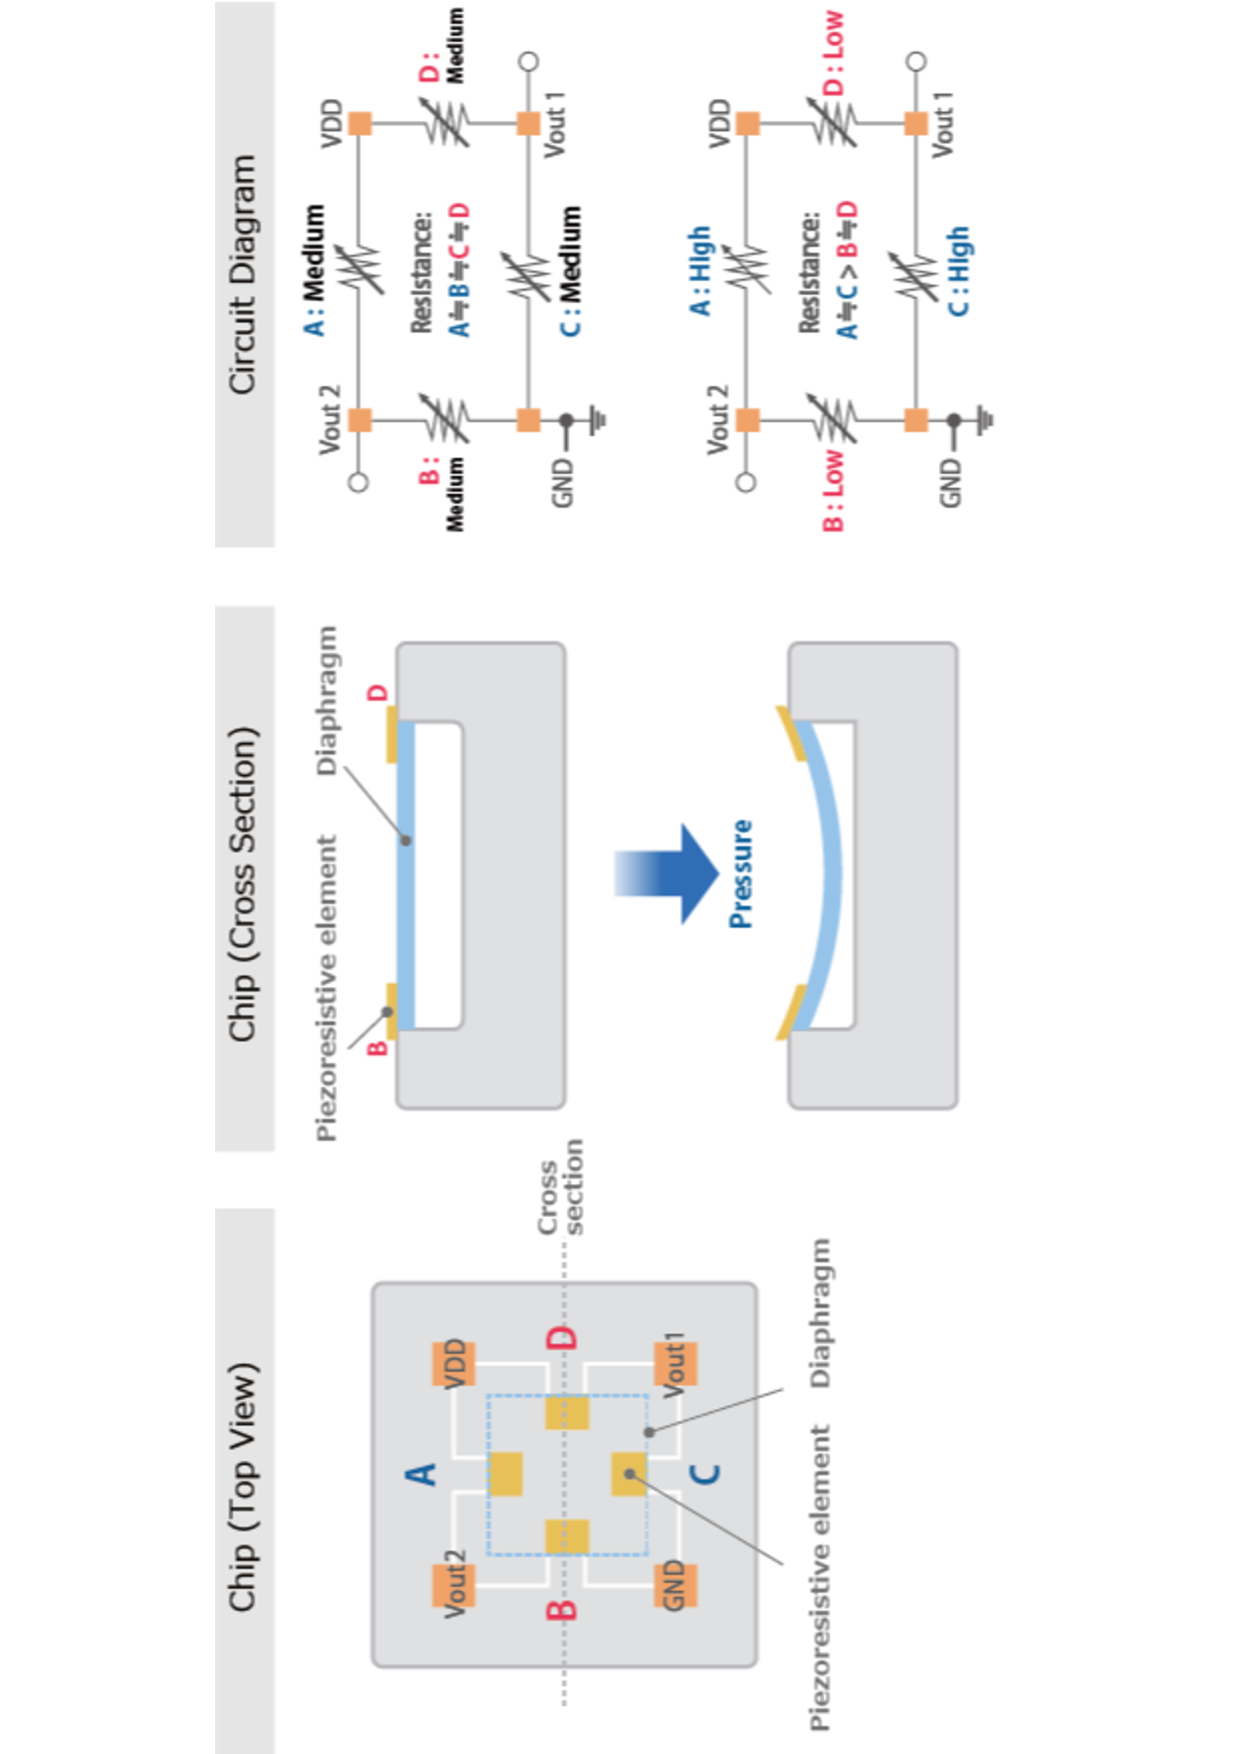
\includegraphics[width=.8\textwidth]{figures/pressureSensor}
        \caption{Principle of a micro-fabricated pressure sensor to measure the barometric pressure
                 of the air. (Alps Alpine)}
        \label{fig:barometer}
    \end{figure}

    \subsection{Acceleration Sensor}
    Accelerometers, as the name itself already says, measures acceleration.
    It does so based on Newton's second law
    \begin{equation}
        F = ma
        \label{eq:newtonsLaw},
    \end{equation}
    by observing the force acting on a mass~\cite{labManual} (seismic mass) which is suspended by springs.
    The position of the mass is read by comb-like structures, and the mass movement results in change in capacity
    between neighboring fingers~\cite{labManual}.

    The typical setup of Micro electromechanical system (MEMS) accelerometers is shown in Figure~\ref{fig:accelerometer}
    \begin{figure}[h]
        \centering
        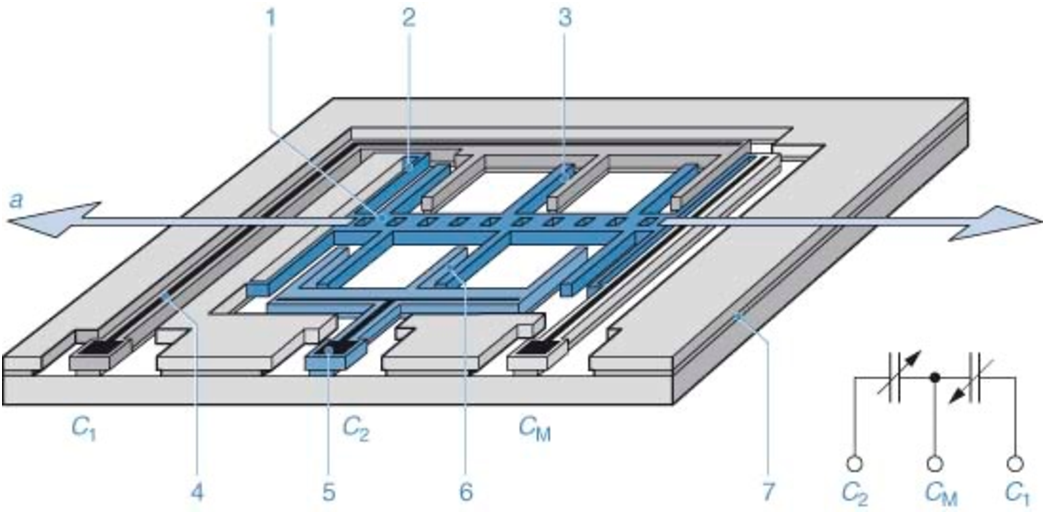
\includegraphics[width=.6\textwidth]{figures/accelerometer}
        \caption{Principle of a microfabricated, capacitive accelerometer to sense the in-plane acceleration (Bosch Gmbh).}
        \label{fig:accelerometer}
    \end{figure}

    \clearpage


    \section{Methods}
    A battery-powered notebook was used to take all measurements from an Arduino Nicla Sense Board ME containing a BHI260AP.
    It was connected to the computer via USB.
    The same notebook was used as a power supply for the board as well as a data logger.
    The board was programmed using the Arduino IDE 2.0.2 with the \texttt{Arduino\_BHY2} library version 1.0.5 (Bosch Sensortec).
    A small MATLAB application called \textit{SampleNicla} was developed to log the data.
    MATLAB was also used to process the data.
    The source code is available in \href{https://github.com/RafasLectures/sensorslab/blob/main/SampleNicla.mlapp}{GitHub}
    (\texttt{https://github.com/RafasLectures/sensorslab/})

    In a \SI{10}{\hertz} sampling rate (every \SI{100}{\milli\second}), the Arduino program reads the acceleration
    virtual sensors \texttt{SENSOR\_ID\_ACC\_PASS} and the barometric sensor
    \texttt{SENSOR\_ID\_BARO} from the BHI260AP.
    The sensitivity of the acceleration sensor was \SI{1670.13}{\frac{\LSB}{\mathrm{m/s^2}}} (2$g$ range) and the
    barometer had a relative accuracy of $\pm$\SI{3}{\pascal} \cite{BHI260}.

    The data acquisition for Task~1 and 2 were performed at the same time.
    The sensor was placed in a flat surface with its $z$-axis pointing upwards (Figure~\ref{fig:setup}).

    For Task~3, the elevator ride was performed in a 5 stories residential building in Freiburg.
    The sensor was placed in the middle of the cabin with its $z$-axis pointing upwards (Figure~\ref{fig:setup}).
    Two rides were performed, one upward and another downwards.
    The first ride started at the lowermost landing up to the 5\textsuperscript{th} floor and the other was the
    other way around.
    The sampling never stopped between the two rides, and before each ride there was a period where the elevator
    stayed in the landing with doors open.

    The measurements of Tasks~1, 2 and 3 were recorded at approximately \SI{20}{\celsius} (indoor).

    \vspace{3em}

    \begin{figure}[h]
        \centering
        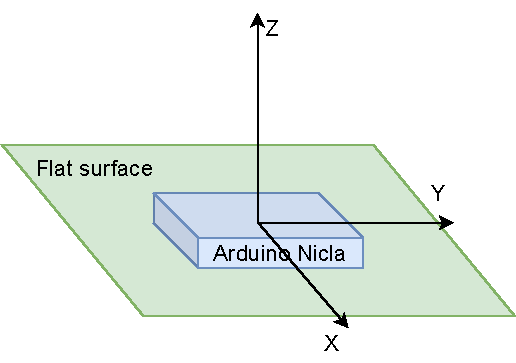
\includegraphics[width=.6\textwidth]{figures/Setup1and2}
        \caption{Setup of Task~1, 2 and 3: the sensor was placed in a flat surface with its $z$-axis pointing upwards
            (author's own work).}
        \label{fig:setup}
    \end{figure}

    \clearpage


    \section{Results and Discussion}

    \subsection*{Task 1}

    The first task is intended to verify the performance of the pressure sensor.
    The noise level is evaluated in this task.
    The Nicla Sense ME Board was placed flat on a steady table and the pressure was recorded.
    The obtained values are in already in \si{\hecto\pascal}.
    No drift is visible.
    Figure~\ref{fig:plotPressure} provides an overview on the 1,000 pressure samples.

    \begin{figure}[h]
        \centering
        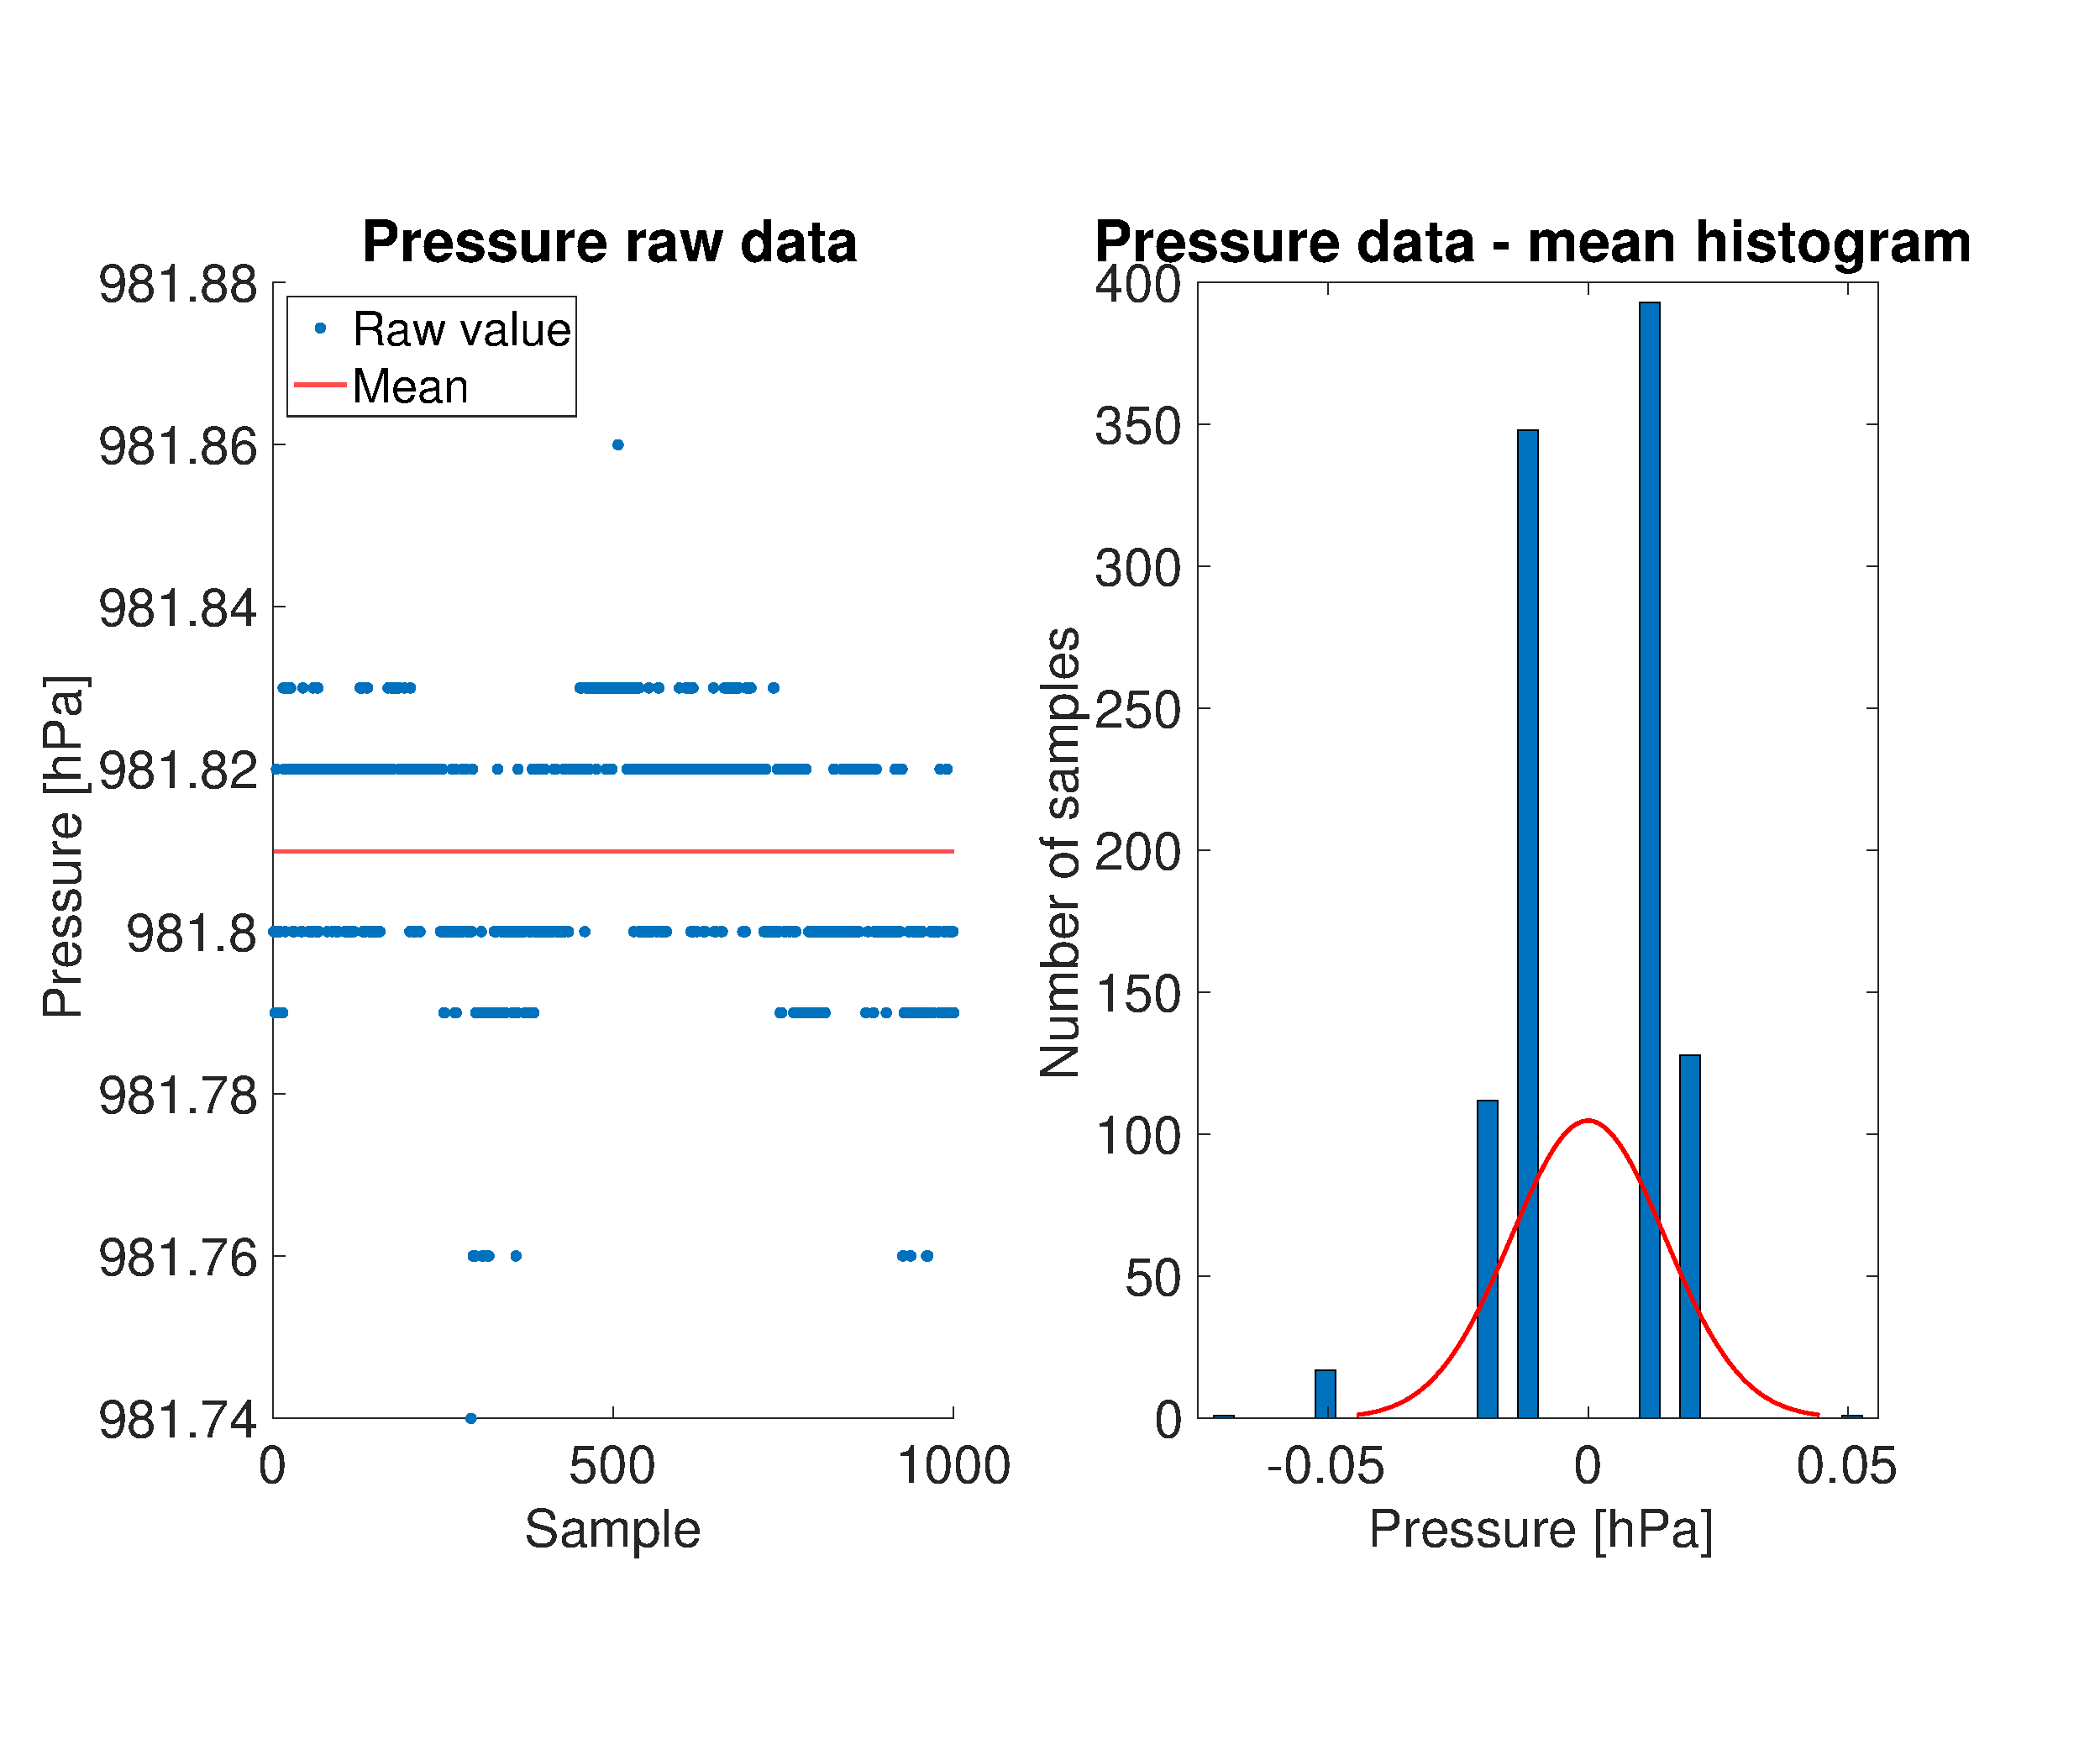
\includegraphics[width=.6\textwidth]{plots/plotPressure}
        \caption{Pressure readings at rest. The measurement rate is \SI{10}{\hertz}.}
        \label{fig:plotPressure}
    \end{figure}

    The mean value $\bar{p}$ is 981.81 \si{\hecto\pascal}.
    It is expected since the pressure at sea level is 1013.25 \si{\hecto\pascal} and we are above sea level,
    so the mean should be slightly below the pressure at sea level.
    The standard deviation $\sigma_p$ is 0.014 \si{\hecto\pascal}
    The histogram shows that the values follow a normal distribution.
    The values are according to the datasheet, which specifies an accuracy of $\pm3 \si{\pascal}$ and
    the standard deviation is within that range.

    \subsection*{Task 2}

    The second task is intended to verify the performance of the accelerometer.
    The noise level and the offset are evaluated in this task.
    The Nicla Sense ME Board was placed flat on a steady table and the acceleration on the $x$, $y$ and $z$-axis were recorded.
    No drift is visible and a small offset is seen on every axis.
    The behaviour of all three axis are the same.
    Table~\ref{tab:accel} shows the offsets.
    Figure~\ref{fig:accelerationHist} shows the raw data together with the histogram of the raw data subtracted by the mean.

    \begin{figure}[h]

        \centering
        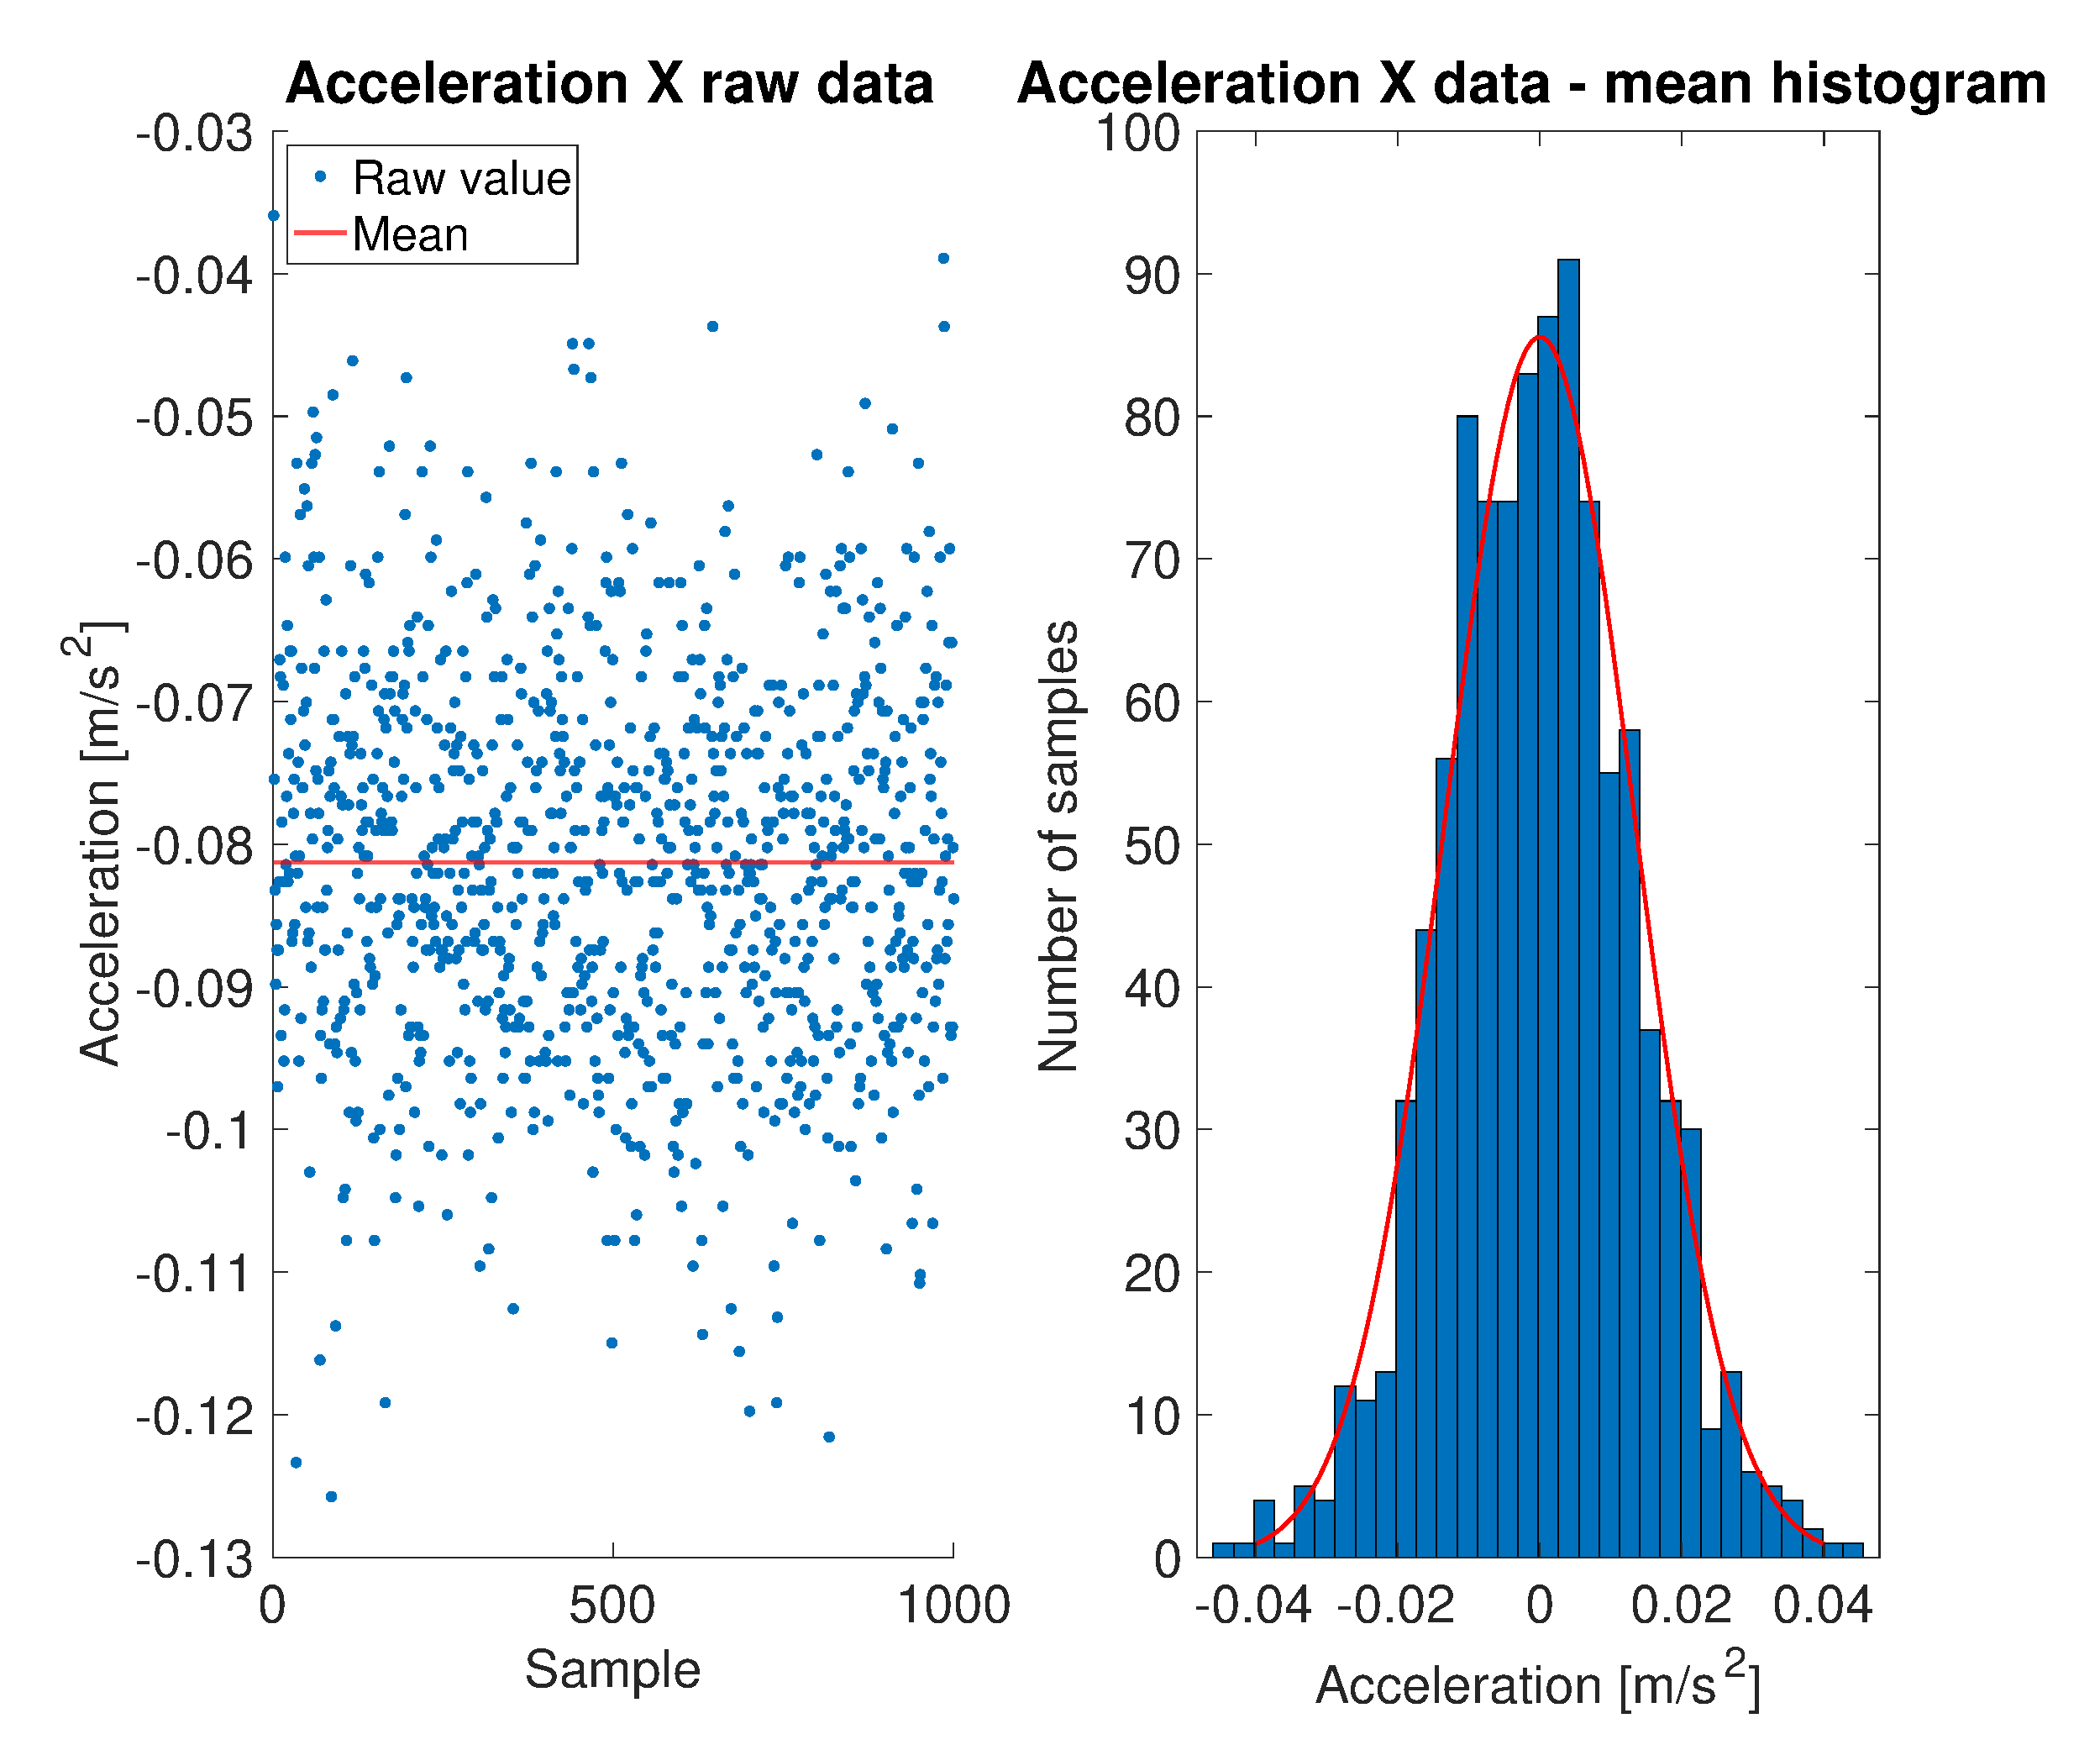
\includegraphics[width=.45\textwidth]{plots/plotAccelerationX}\hfill
        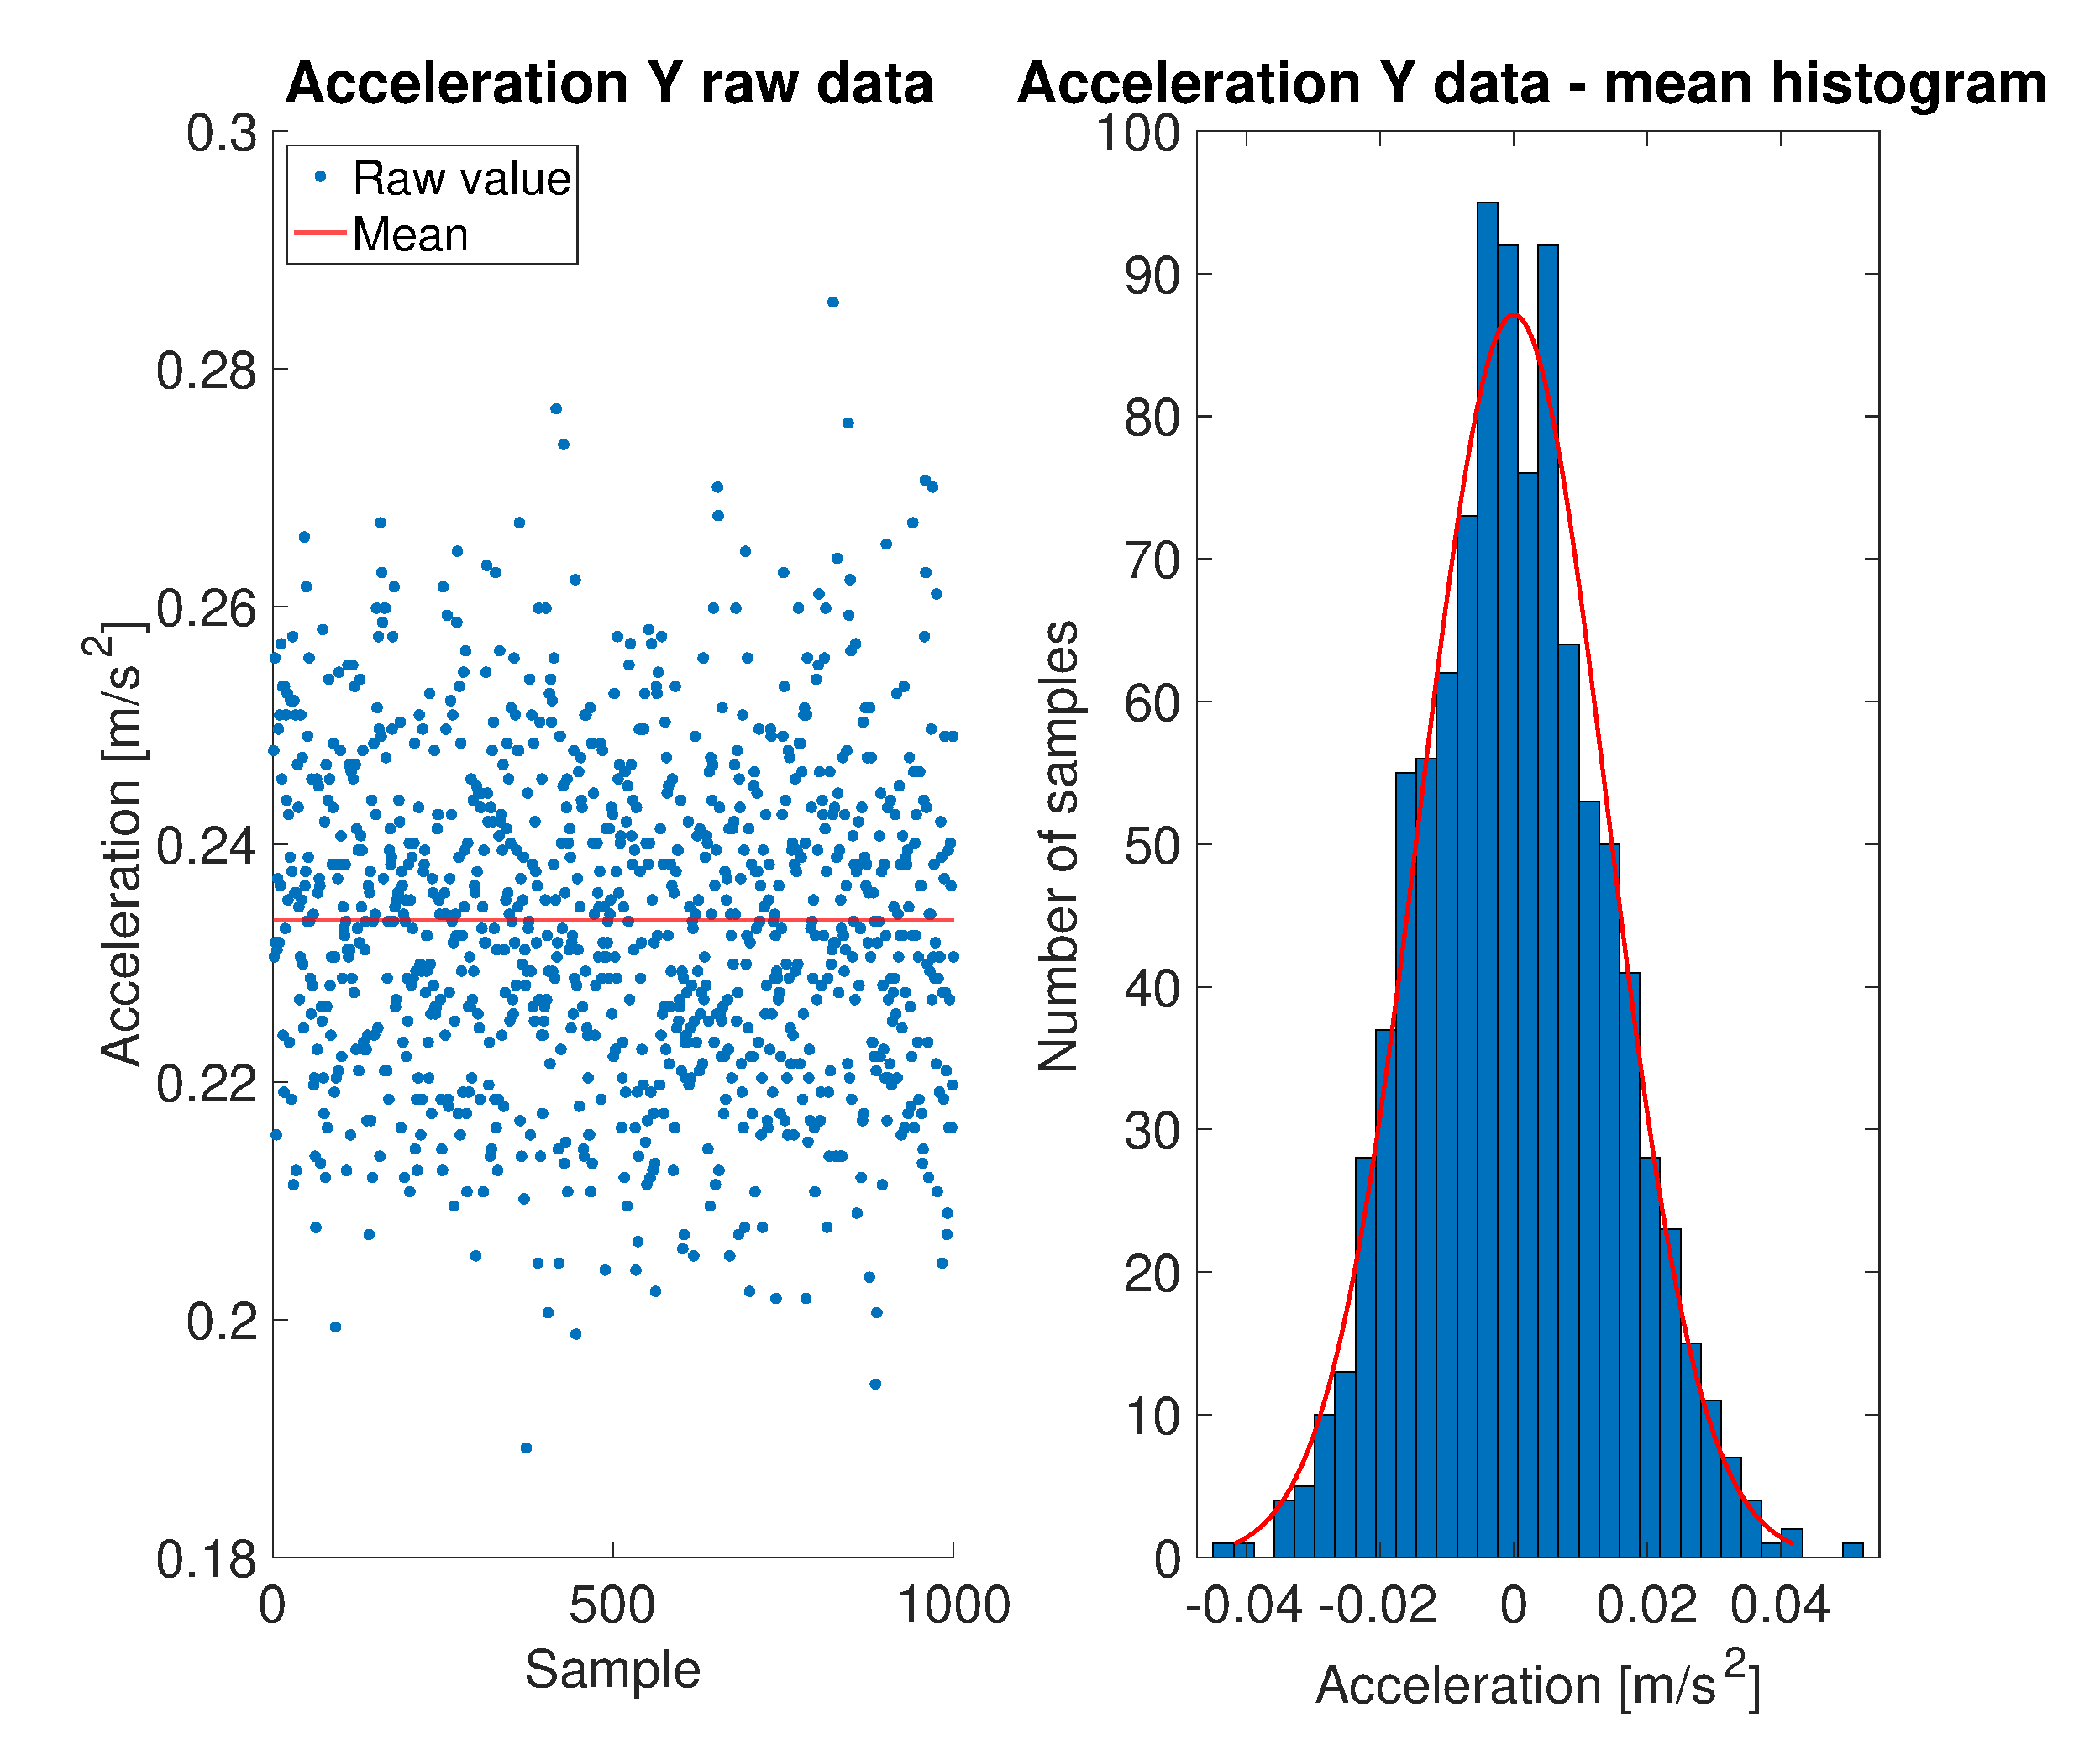
\includegraphics[width=.45\textwidth]{plots/plotAccelerationY}\vspace{1em}
        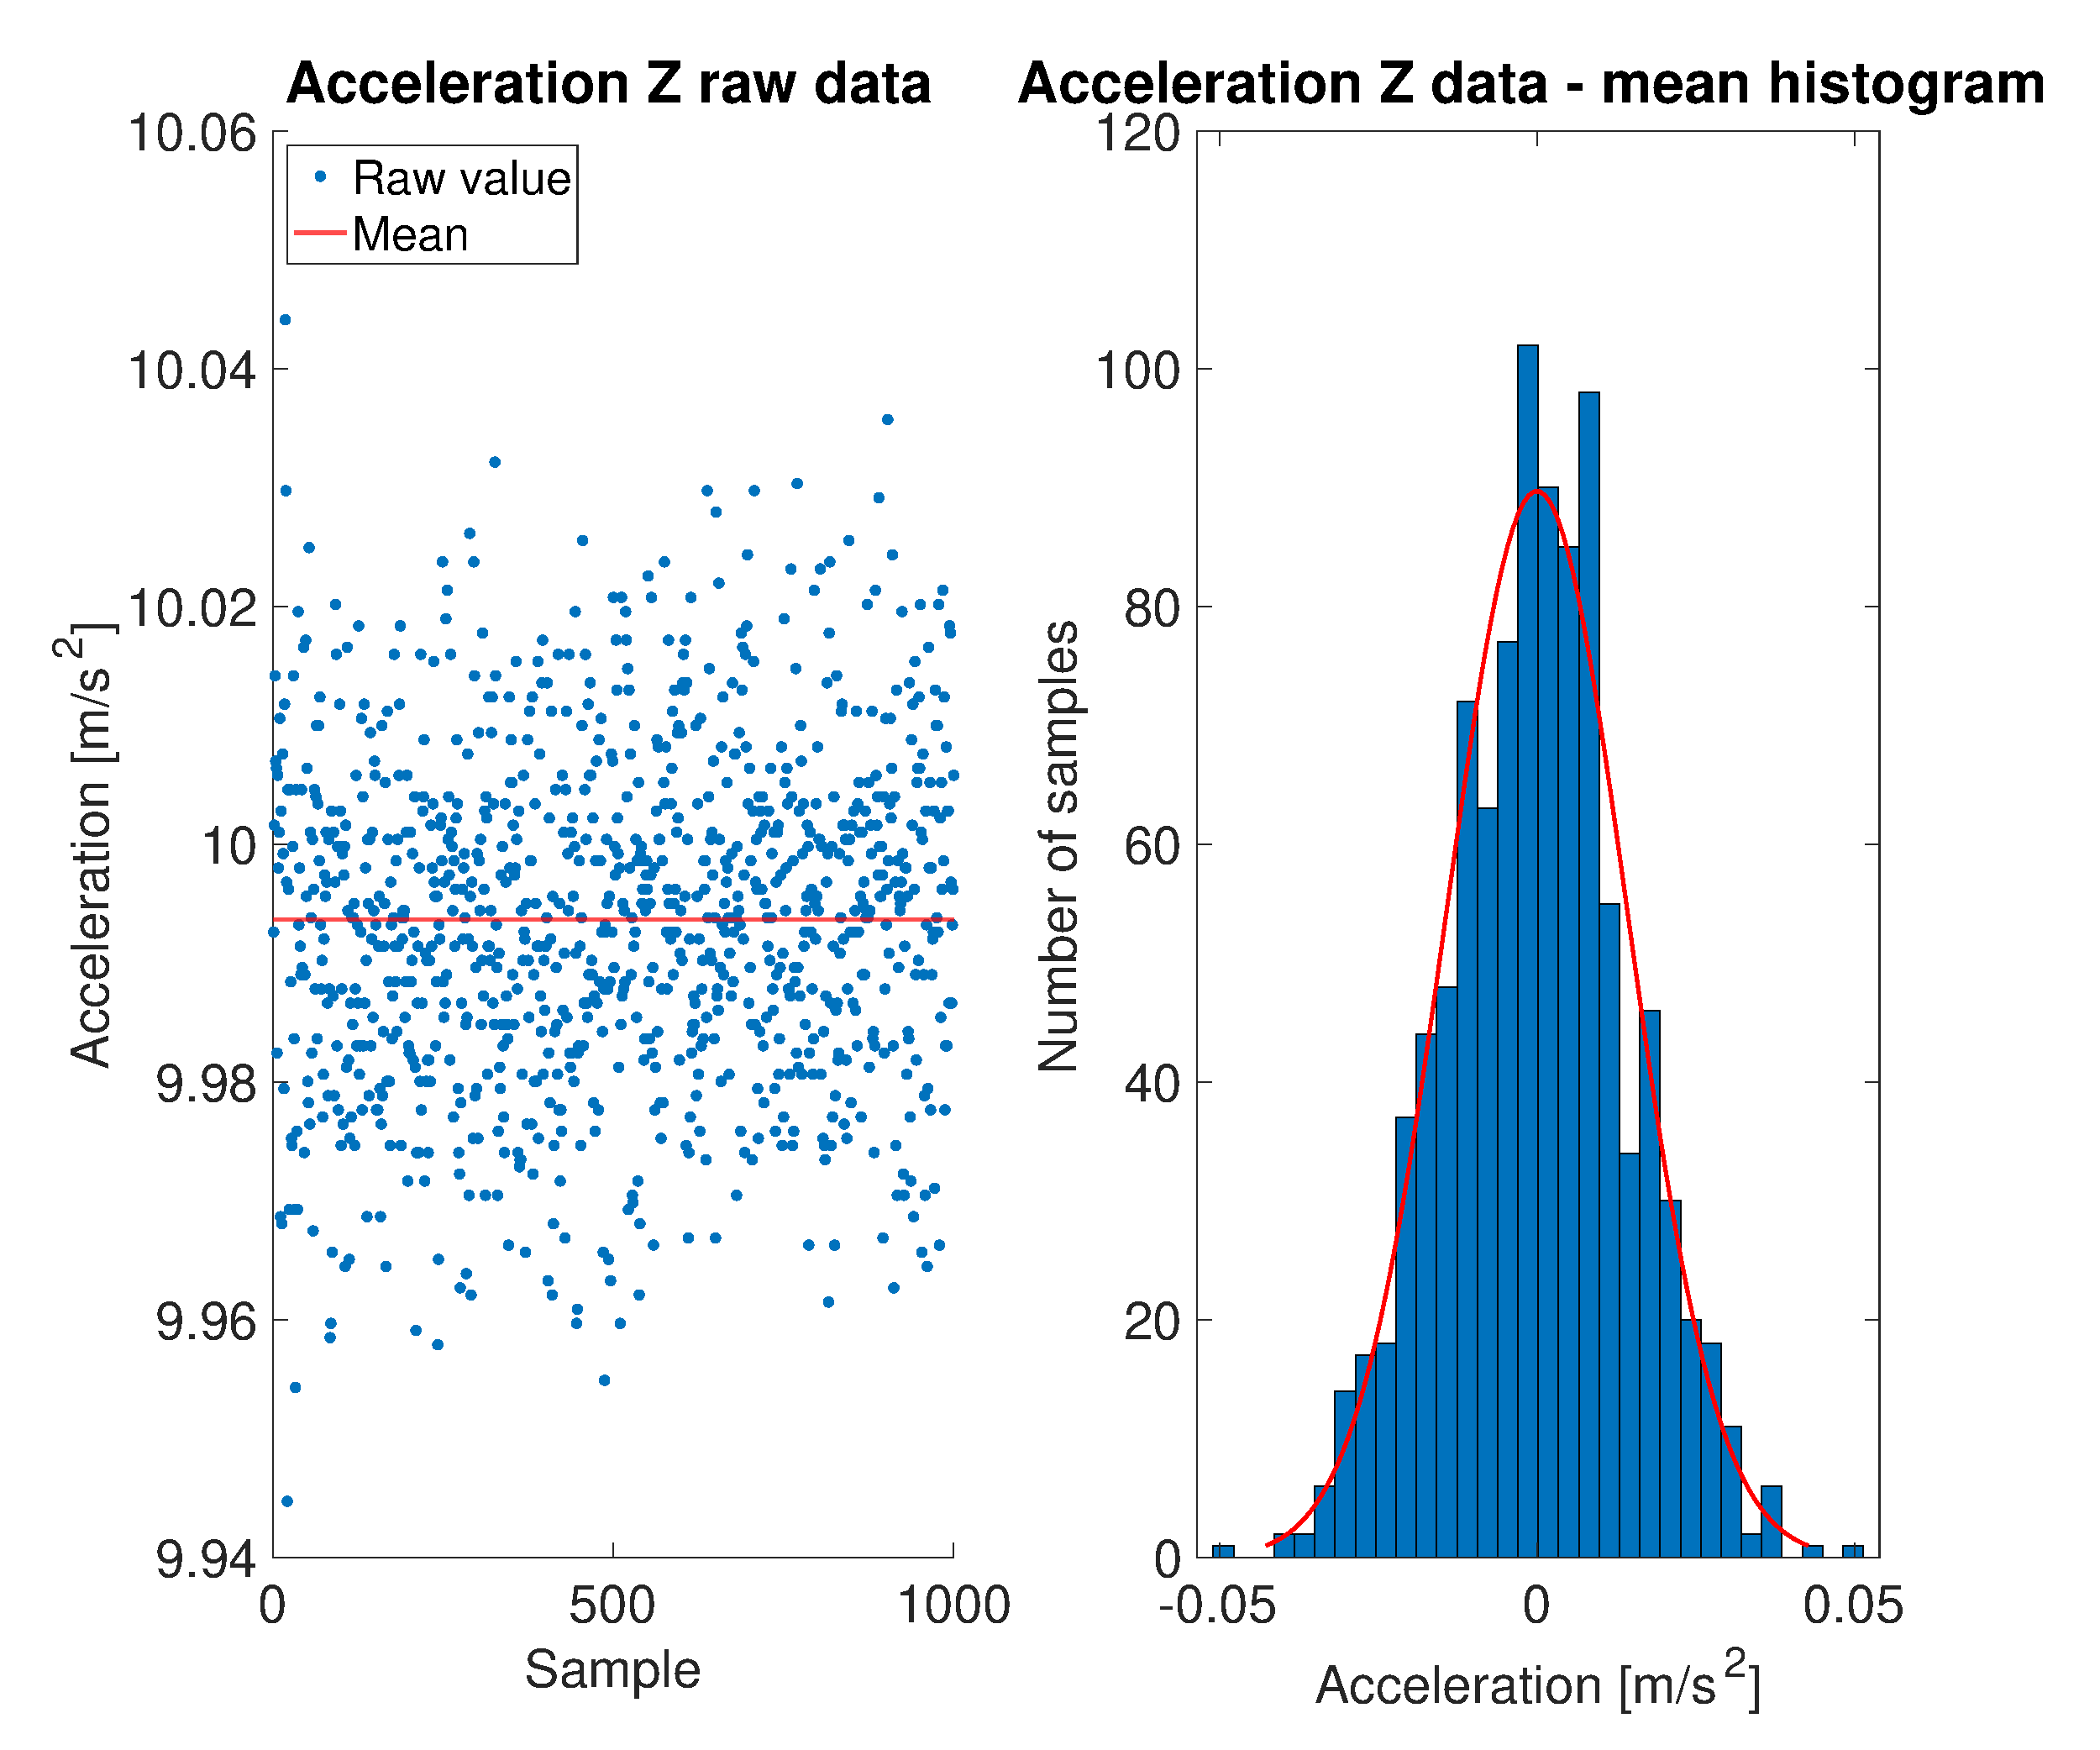
\includegraphics[width=.45\textwidth]{plots/plotAccelerationZ}\hfill
        \caption{Scatter raw data and histograms of the accelerometer reading at rest with subtracted offset. All three directions allow approximation by a normal distribution.}
        \label{fig:accelerationHist}
    \end{figure}


    They follow a normal distribution with the mean ($\bar{\mathit{a}}$) and standard deviation($\sigma_a$) shown in table~\ref{tab:accel}
    The offset of the $z$-axis was calculated by removing the gravity (9.81) from its mean.
    The reason for that is because the $z$-axis is actually measuring gravity.
    If another axis was placed in the same axis to gravity, one could see the offset in the $z$-axis.
    Since the gravity is known, its value was simply subtracted from the mean in the $z$-axis.

    \begin{table}[!ht]
        \centering
        \begin{tabular}{cS[table-format=1.3]S[table-format=1.3]S[table-format=1.3]}
            \hline \vspace{-1em} \\
            Direction & {Offset in \si{\meter\per\second\squared}} & {$\bar{\mathit{a}}$ in \si{\meter\per\second\squared}} & {$\sigma_a$ in \si{\meter\per\second\squared}} \\ \hline
            $x$       & -0.0812                                    & -0.0812                                                & 0.0013                                         \\
            $y$       & 0.2335                                     & 0.2335                                                 & 0.0013                                         \\
            $z$       & 0.1836                                     & 9.9936                                                 & 0.0014                                         \\ \hline
        \end{tabular}
        \caption{Summary of the acceleration readings at rest. The number of samples was 1,000 in each direction.
        Please note the quantization of \SI{0.00059}{\meter\per\second\squared} for the individual values.}
        \label{tab:accel}
    \end{table}

    The datasheet specifies a zero-$g$ offset of $\pm20 \mathrm{mg} \approx 0.196\si{\meter\per\second\squared}$.
    When looking at the computed offset from the measurements, we see that they are consistent to the datasheet.

    \subsection*{Task 3}
    Task three was intended to measure the acceleration and pressure during an elevator ride.
    The Nicla Sense ME Board was placed in on the floor, in the middle of the elevator cabin
    and the acceleration and pressure were recorded during a ride from floor 0 to floor 4 and back.
    Before starting to move, the elevator remained stopped with open doors, enabling me to take the
    average of the acceleration before the beginning of the ride.
    The measured pressure and acceleration are shown in Figure~\ref{fig:plotElevatorRaw}

    \begin{figure}[h]
        \centering
        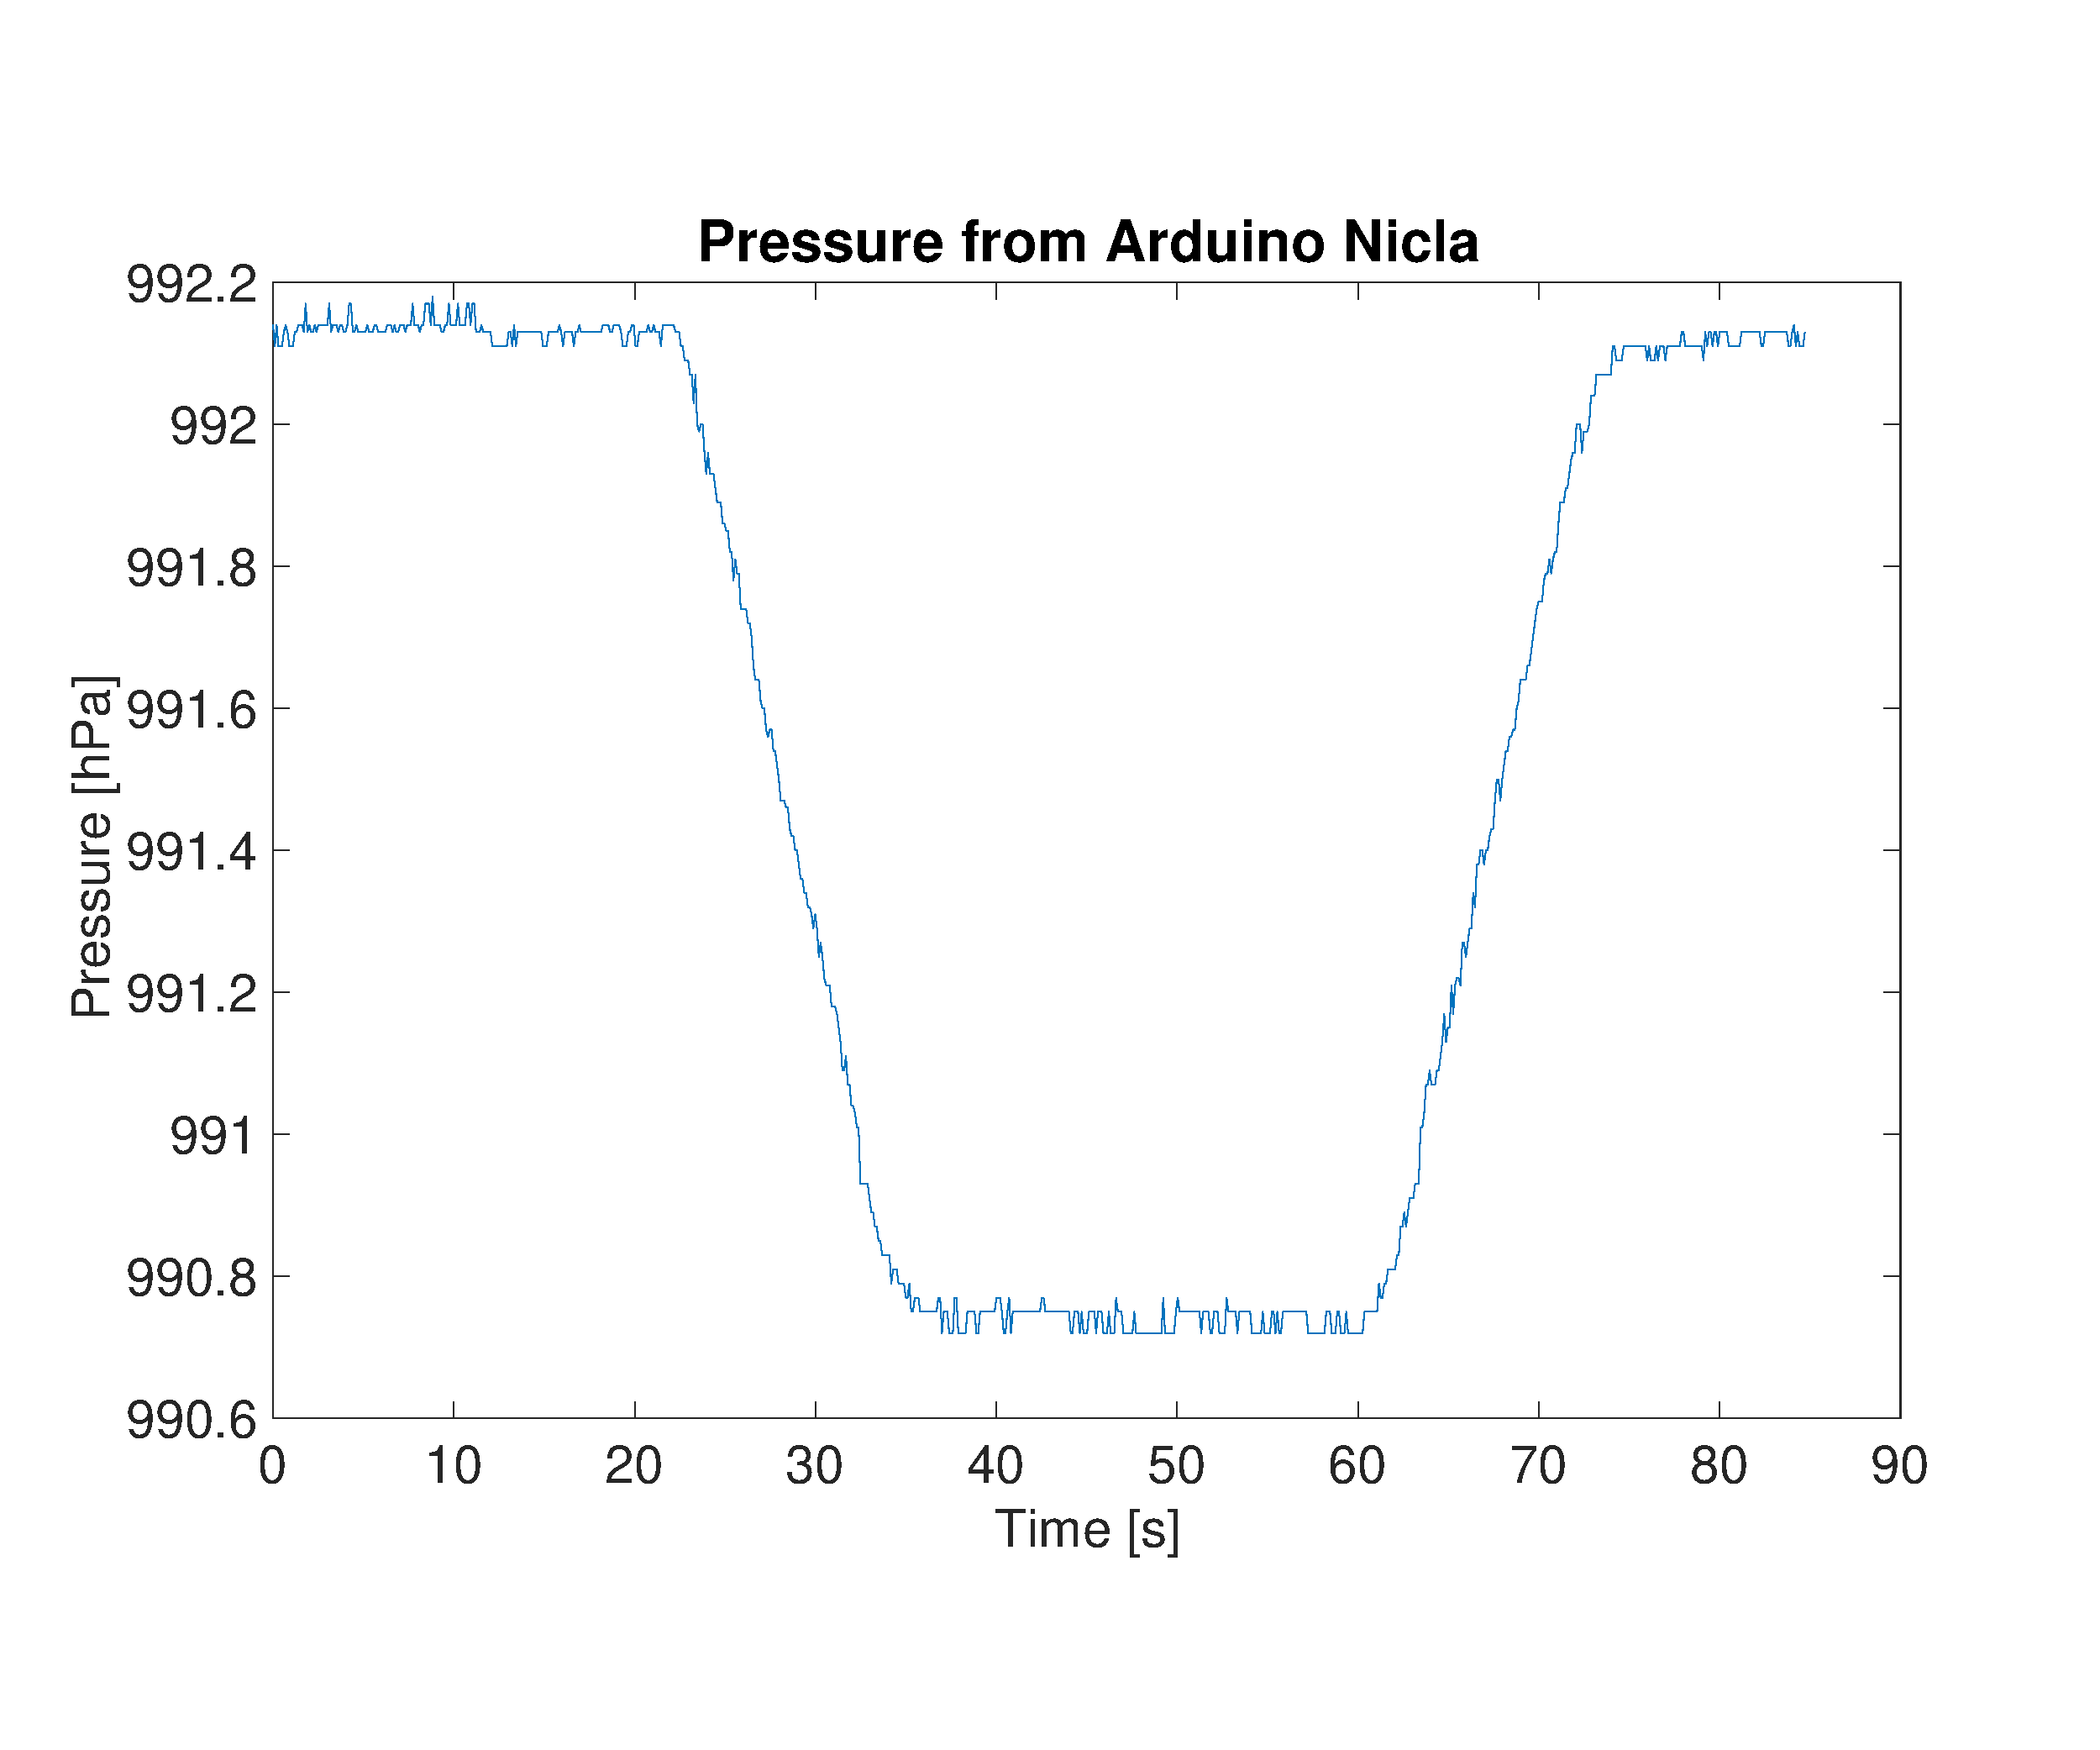
\includegraphics[width=.5\textwidth]{plots/plotElevatorPressure}\hfill
        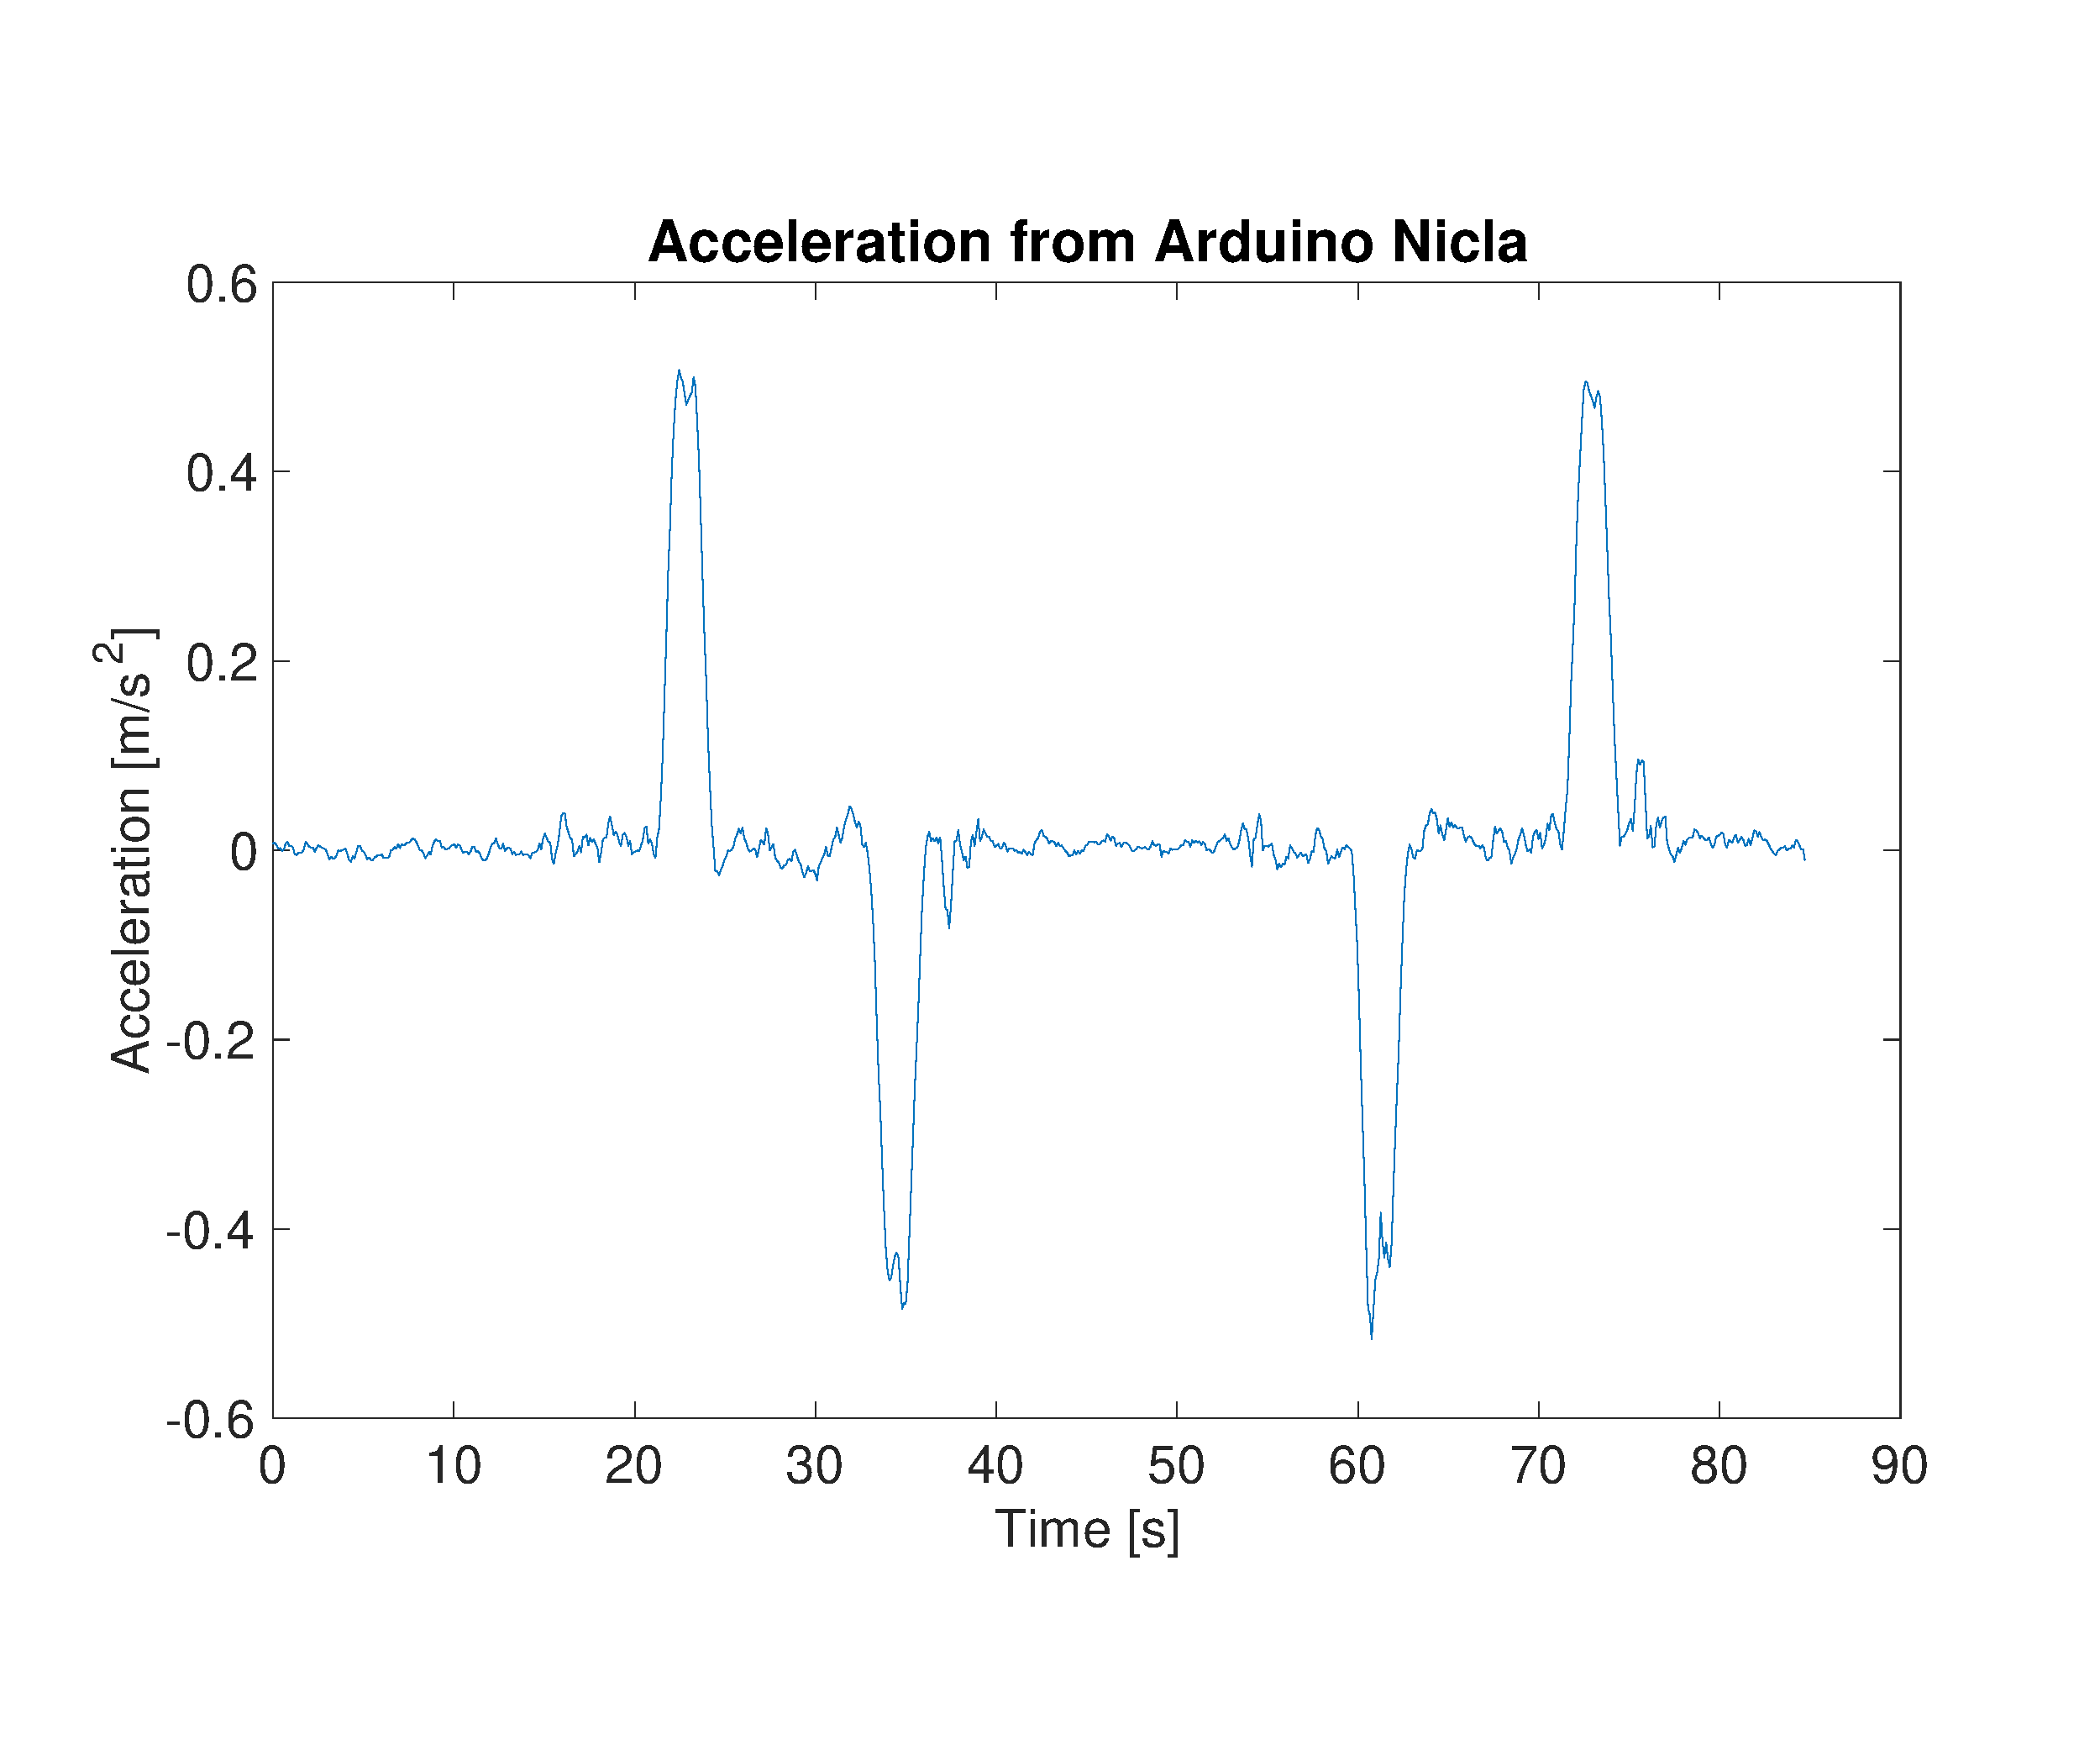
\includegraphics[width=.5\textwidth]{plots/plotElevatorAcceleration}\hfill
        \caption{Measured data during elevator ride. Pressure in \si{\hecto\pascal} and acceleration in
        \si{\meter\per\second\squared}. Acceleration was smoothed with a moving average of 5 samples (0.5 seconds)}
        \label{fig:plotElevatorRaw}
    \end{figure}

    During the upwards movement we can see that we first accelerate, and then decelerate.
    In the downwards movement it is the opposite, first decelerate, then accelerate.
    During the deceleration of the second ride, one can see a very big peak during the constant deceleration phase.
    The reason for it can be the combination of a bad regulated motor controller added up to noise,
    since the same feature with different amplitudes is seen in every constant acceleration and deceleration phases.

    Using the pressure equation (Equation~\ref{eq:relativePressureHeight}) one can calculate the relative height of the
    elevator.
    The mean pressure was taken from the first 11 seconds of the recording, this value was used as $p_1$ and the current
    measured pressure was used as $p_2$.
    The resulting conversion from pressure to height, is seen in Figure~\ref{fig:plotElevatorPressureHeight}

    \begin{figure}[!h]
        \centering
        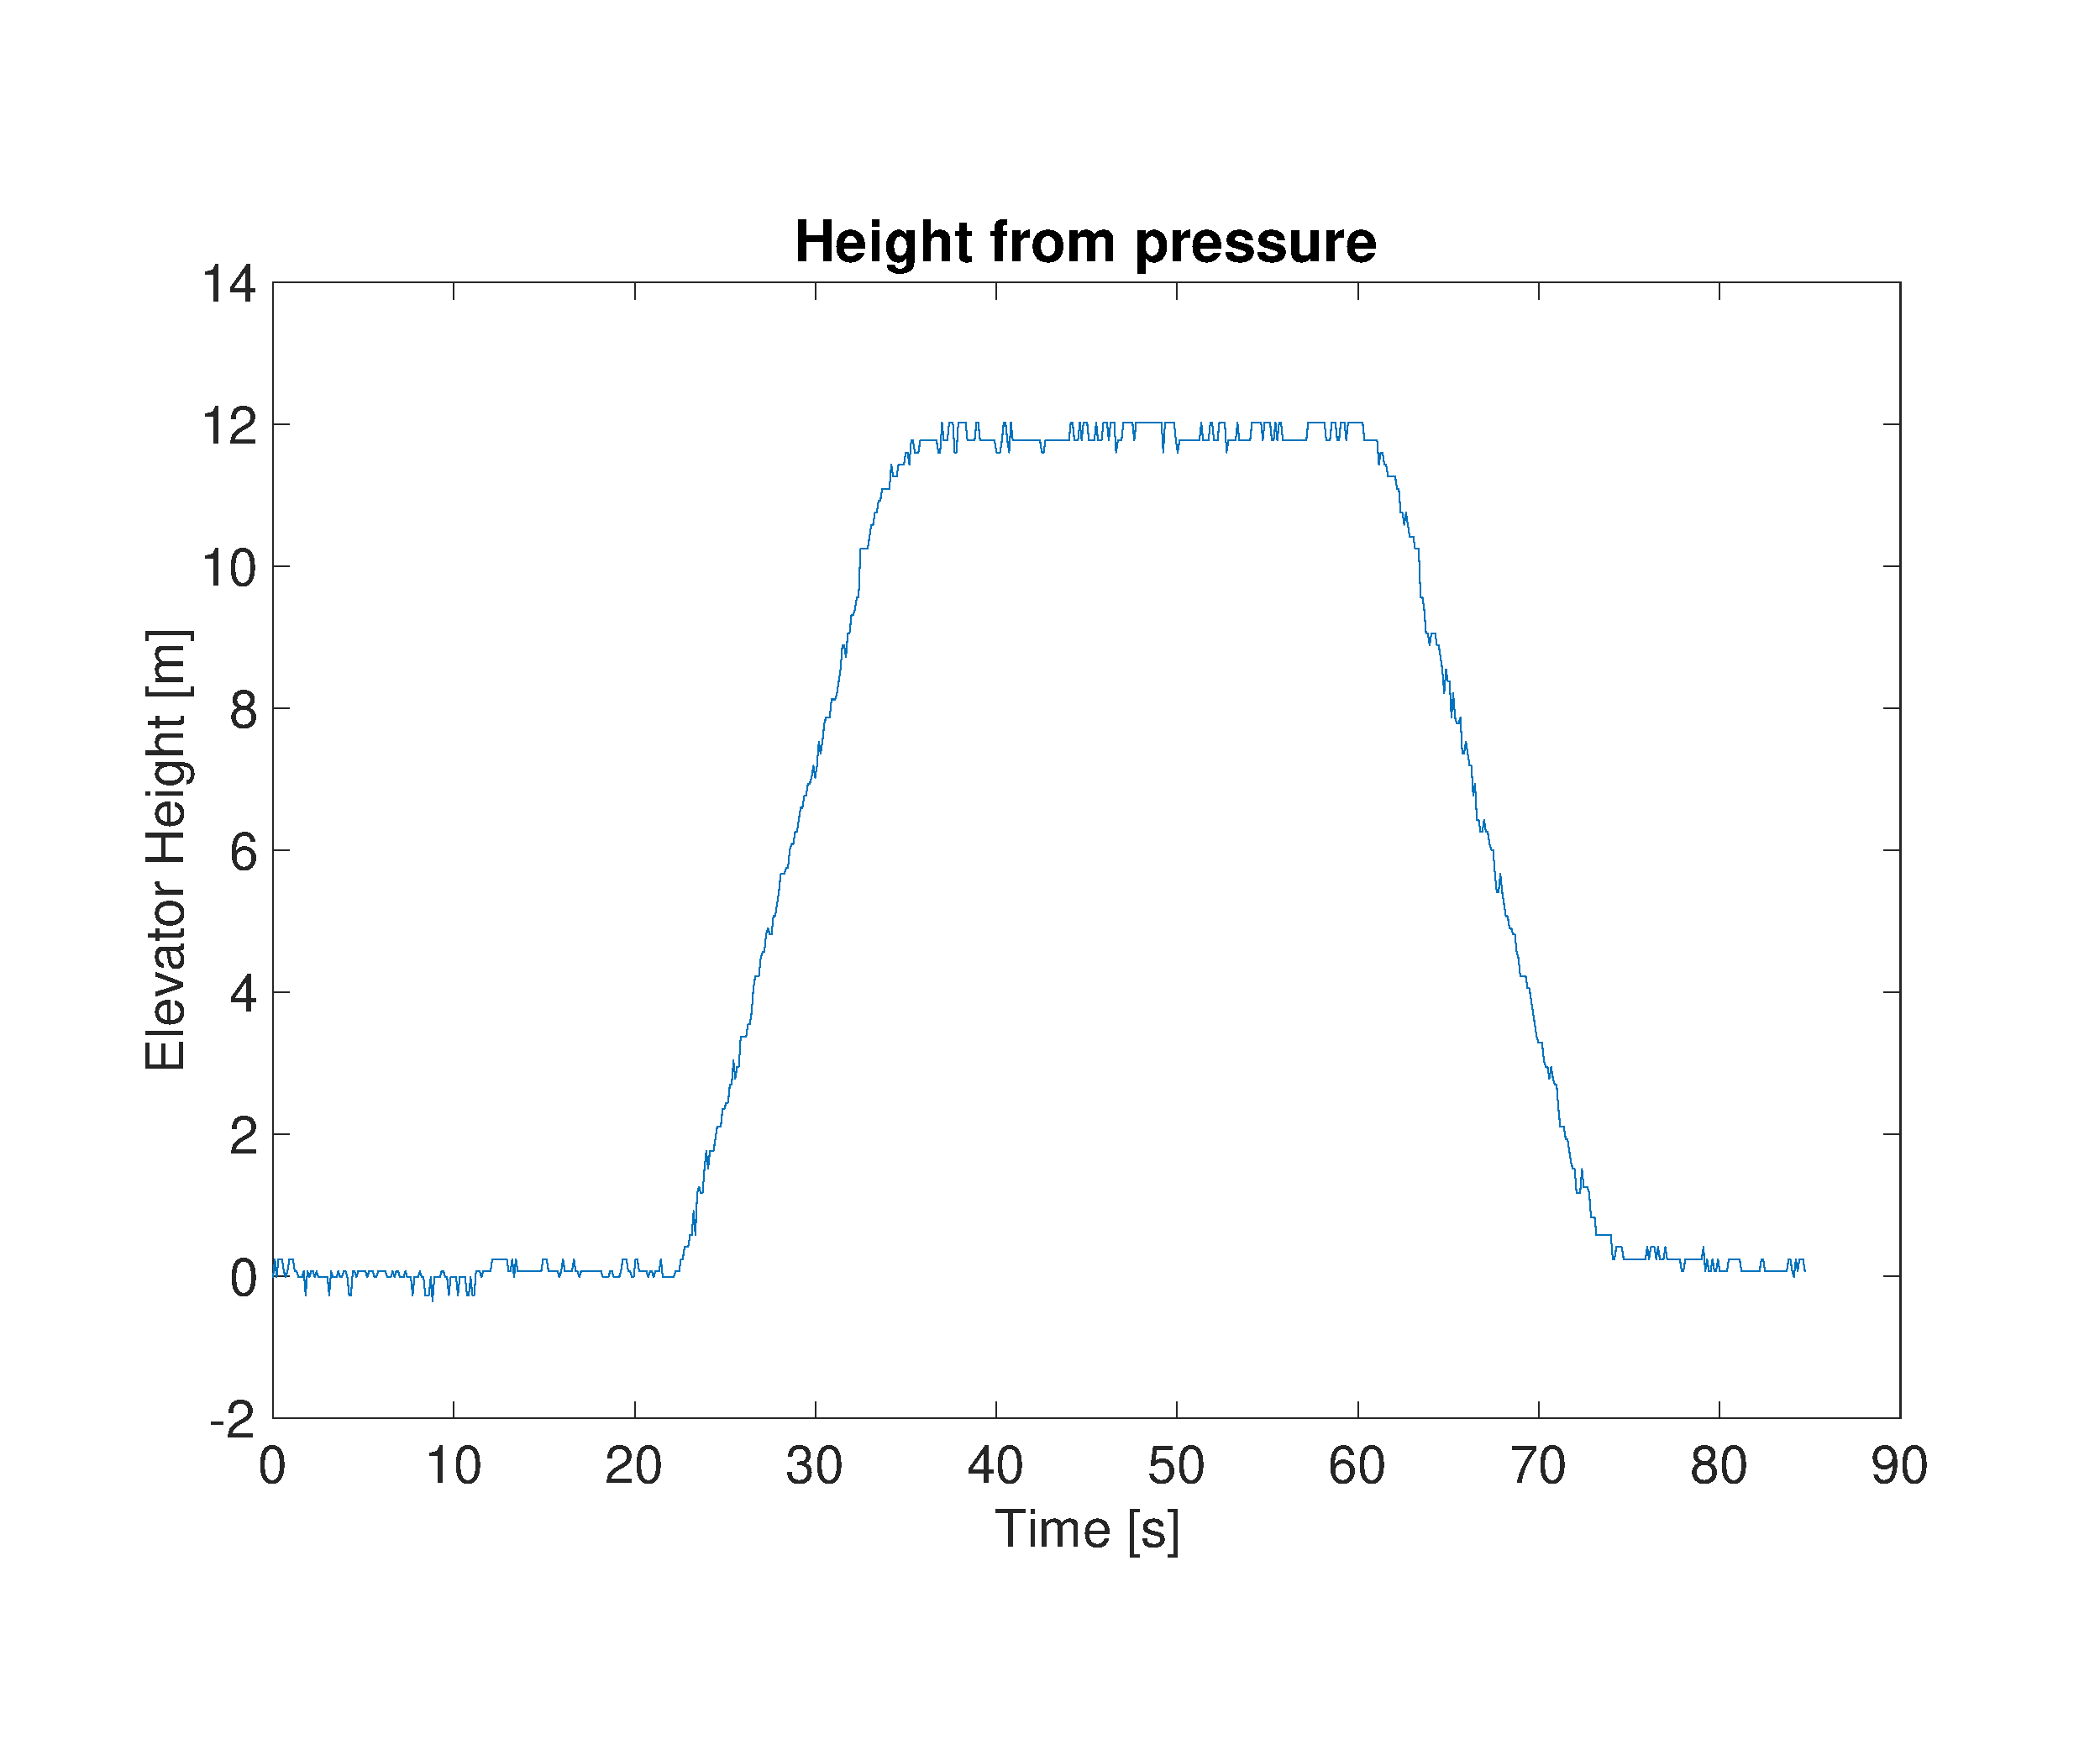
\includegraphics[width=.6\textwidth]{plots/plotElevatorPressureHeight}
        \caption{Result of conversion from pressure to height.}
        \label{fig:plotElevatorPressureHeight}
    \end{figure}

    The result seems to be realistic, since we can estimate $\pm3$ meters per floor, and we go up 4 floors.

    As seen in section~\ref{sec:theory} one can integrate the acceleration to obtain the speed, and integrate twice to
    obtain the position.
    Firstly the acceleration was smoothed using a moving average of 5 samples (0.5 seconds), and after the smoothening,
    the velocity was obtained by integrating the acceleration with a cumulative trapezoidal numerical
    integration method (function \texttt{cumtrapz} in MATLAB).
    The position was obtained by integrating the resulting velocity using the same method.
    The result of it is shown in Figure~\ref{fig:plotElevatorVelocityAndPosition}.

    \begin{figure}[h]
        \centering
        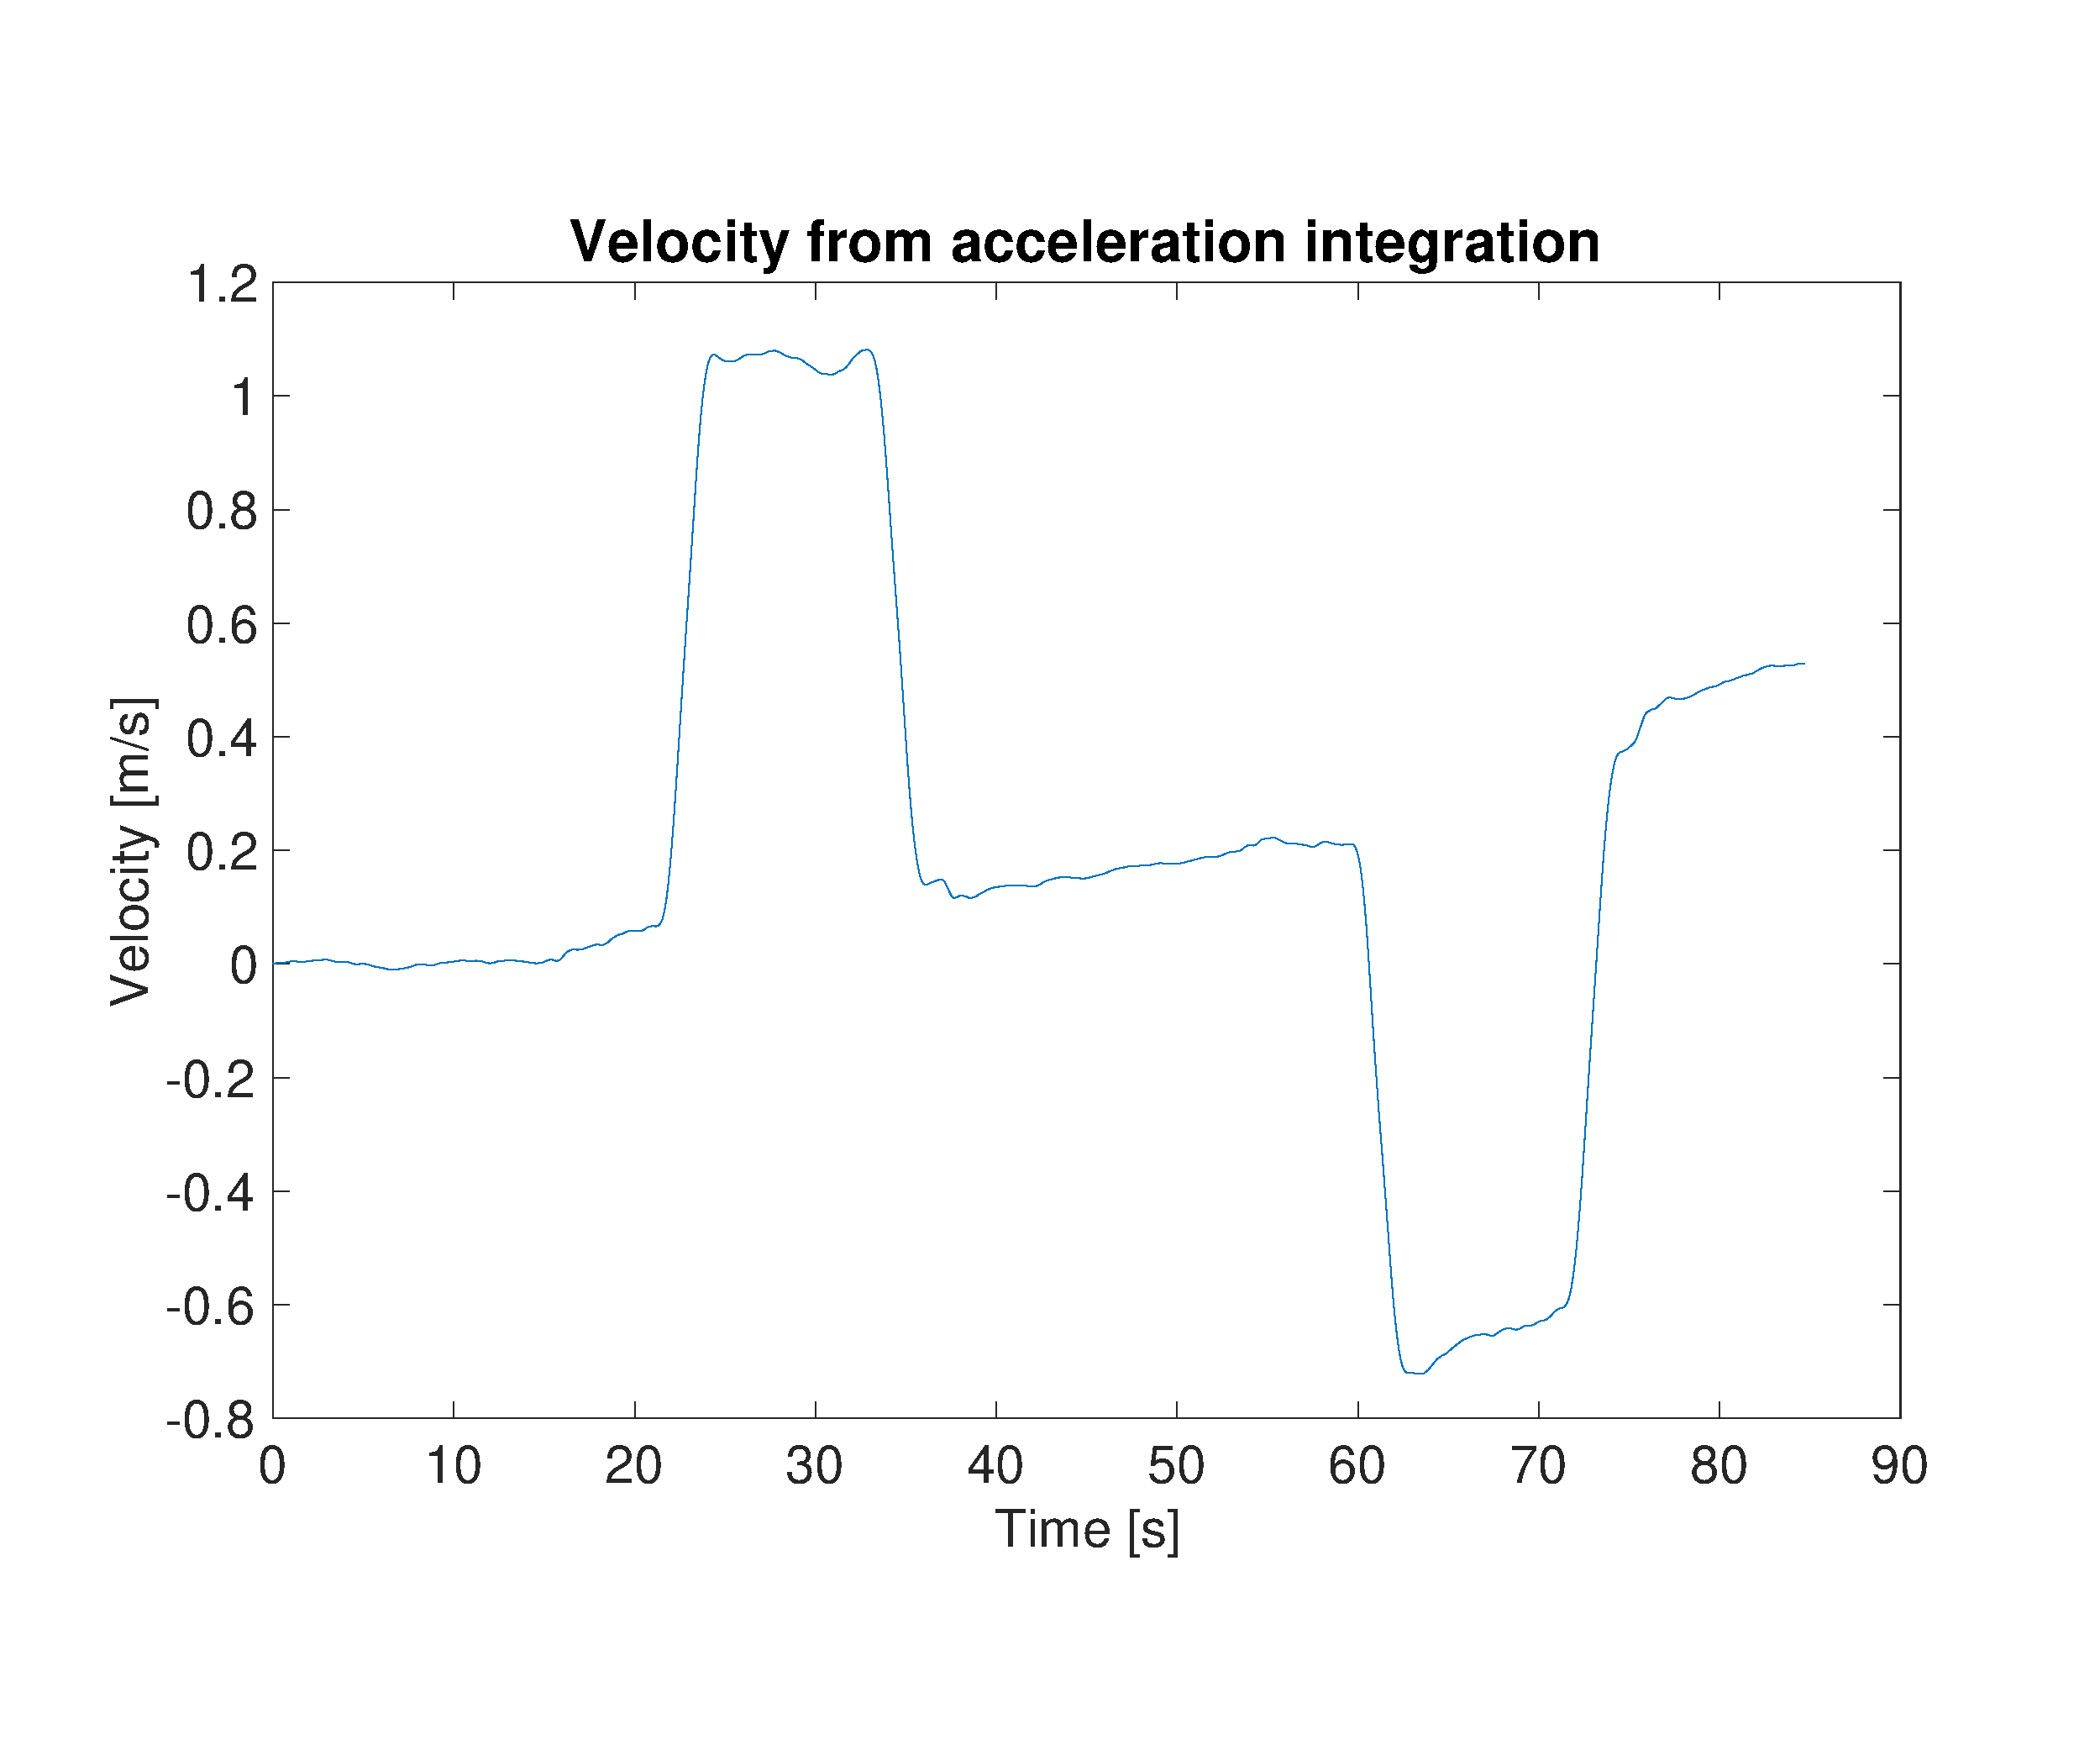
\includegraphics[width=.5\textwidth]{plots/plotElevatorVelocity}\hfill
        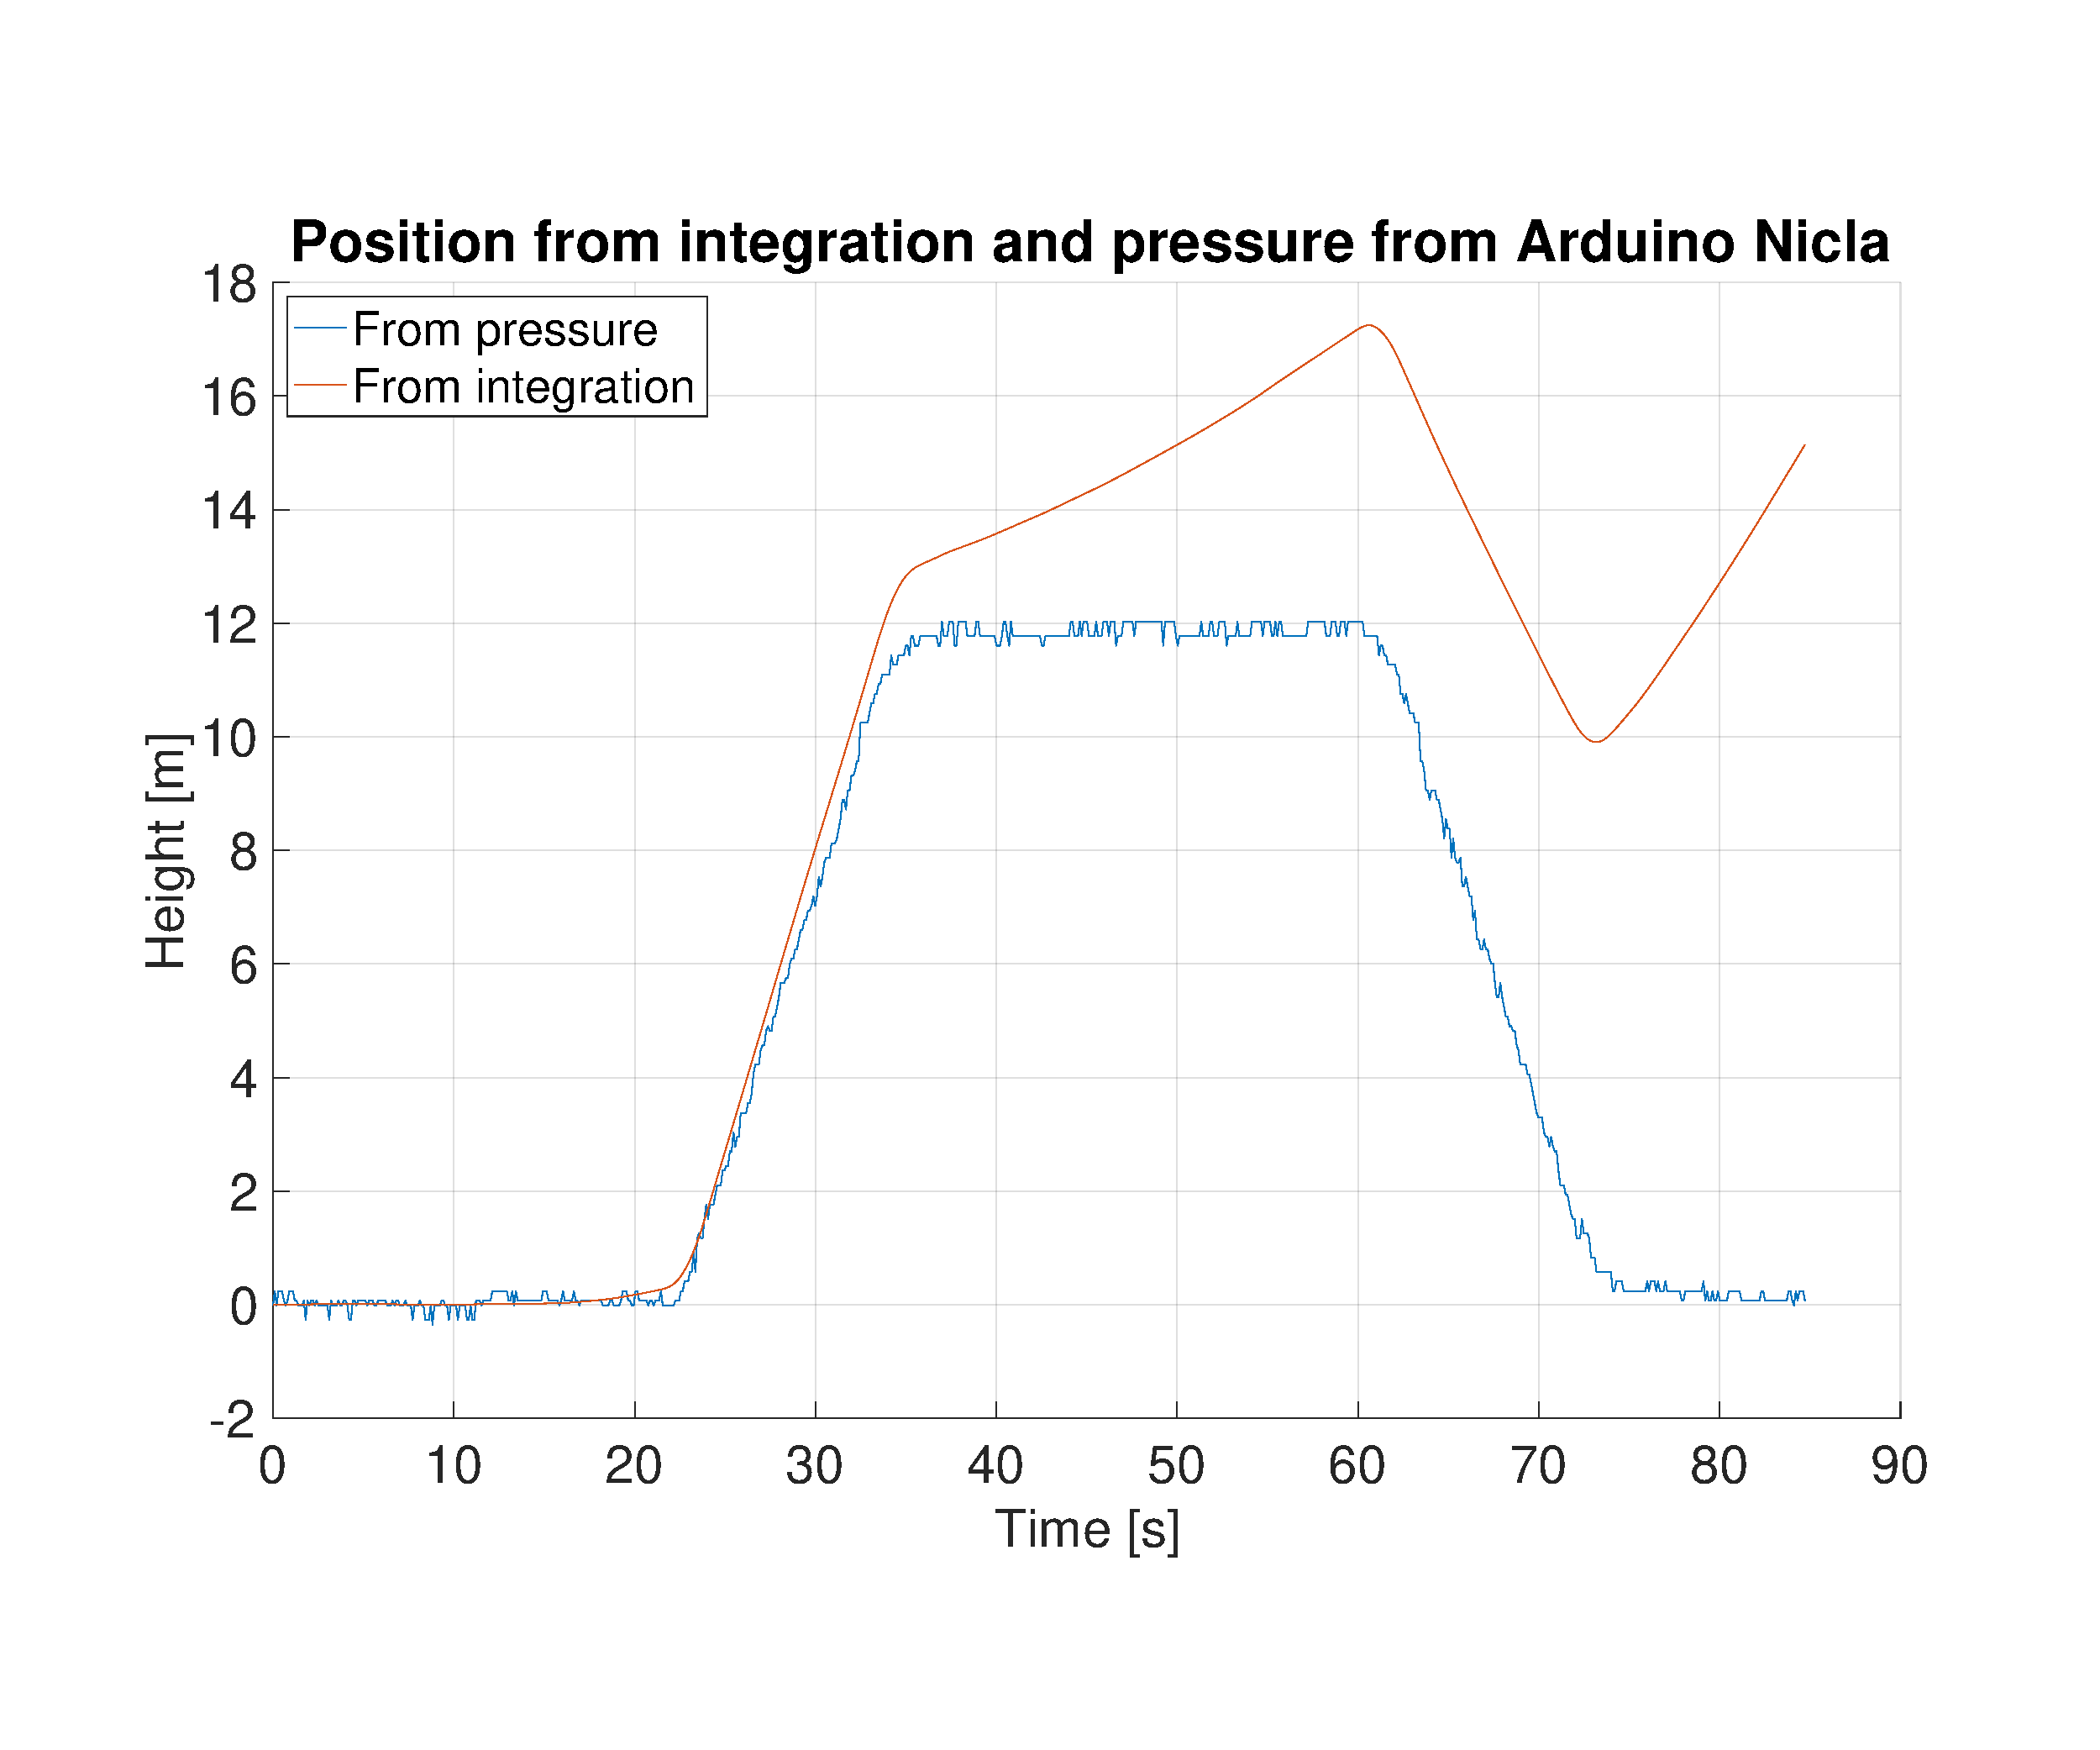
\includegraphics[width=.5\textwidth]{plots/plotElevatorPositionFromIntegrationAndPressure}\hfill
        \caption{Result of integration of acceleration to get velocity and comparison between height obtained from
        two integrations and pressure. Acceleration was smoothed with a moving average of 5 samples (0.5 seconds)}
        \label{fig:plotElevatorVelocityAndPosition}
    \end{figure}

    \subsubsection*{Comparison}
    Clearly, the height measurement is more reliable when we obtain from the pressure sensor.
    The reason is that the acceleration errors are integrated twice, and they accumulate over time, while this is not the
    case for the pressure sensor height prediction.
    An even better approach could be to combine both sensors, such as when we detect acceleration less than a specific
    threshold and the pressure is constant we could set the velocity to zero, and set a constant position.

    \section{Summary}
    Experiments show that the pressure sensor displays no drift.
    The acceleration sensor has a very small offset and has no drift, as well as there were no difference observed
    between the three axes.
    During the elevator ride, the accelerometer and barometer showed realistic values.
    Measuring the height with the barometer is better than integrating the acceleration twice.


% BibTeX or Biber would be better options, with just 2 reference the "raw" approach is fine for such a report
    \begin{thebibliography}{------}

        \bibitem[1]{labManual} J. Kieninger, S.\,J. Rupitsch, \textit{Sensors Lab Course}.
        University Freiburg.
        Winter term 2022/23.

        \bibitem[2]{BHI260} \textit{BHI260AP Datasheet}, Bosch Sensortec, BST-BHI260AP-DS000-02, rev. 1.1, 15-Apr-2021.
        \bibitem[3]{Hautala} Hautala, S., \textit{Physics Across Oceanography: Fluid Mechanics and Waves},
                             Available: https://uw.pressbooks.pub/ocean285/chapter/the-pgf/. [Accessed: 27-Nov-2022]
        \bibitem[4]{alpsAlpine} https://tech.alpsalpine.com/e/products/faq/images/landing/piezo_lp_01_03.png [Accessed:02-Dez-2022]

    \end{thebibliography}


\end{document}
